%% =====================================================================
%%  International Journal of Production Research (IJPR) -- version 2
%%  Taylor & Francis "Interact" layout, APA reference style.
%%
%%  This version supersedes IJPR_CSLAP.tex. It carries the complete,
%%  up-to-date study (multi-instance synthetic benchmark with the
%%  set-partitioning column generation and the LPT anchor, the revised
%%  industrial case with the station-indexed column-generation run, the
%%  temporal hold-out, and the bounded-reassignment sweep).
%%
%%  Compile with the official "Taylor & Francis Interact (APA)" bundle:
%%  keep interact.cls in the working folder (it ships with the template),
%%  together with this file and IJPR_CSLAP.bib. On Overleaf, start from
%%  the "Taylor & Francis Interact (APA reference style)" template and
%%  replace its main.tex and .bib with these two files.
%%
%%  References use BibTeX via apacite (natbibapa), exactly as documented
%%  in the template's main.tex; bibliographystyle = apacite (set below).
%%  Do NOT also load natbib: apacite's natbibapa option provides
%%  \citep / \citet.
%% =====================================================================
% Ensure the "table" option reaches xcolor no matter which package pulls it in
% first (tikz also loads xcolor); this avoids an option clash.
\PassOptionsToPackage{table}{xcolor}
\documentclass[]{interact}

% interact.cls already loads amsmath, amssymb, amsfonts, amsthm, booktabs,
% epsfig, graphicx and rotating. We add only what this manuscript needs.
\usepackage{mathtools}
\usepackage{multirow}
\usepackage{float}
\usepackage{xcolor}  % "table" option passed above; enables \rowcolor/\cellcolor
\usepackage{algorithmicx}
\usepackage{algorithm}
\usepackage{algpseudocode}
\usepackage{tabularx}
\usepackage{colortbl}
\usepackage{xltabular}



% Removes vertical gaps introduced by booktabs around colored rows
\setlength{\aboverulesep}{0pt}
\setlength{\belowrulesep}{0pt}

\usepackage{booktabs}
\usepackage{tikz}
\usetikzlibrary{shapes.geometric, arrows.meta, positioning, calc}
\usepackage{url}
\usepackage{hyperref}

% APA references via BibTeX, exactly as the interact-APA sample documents.
\usepackage[natbibapa,nodoi]{apacite}
\setlength\bibhang{12pt}
\renewcommand\bibliographytypesize{\fontsize{10}{12}\selectfont}

\begin{document}

\articletype{RESEARCH ARTICLE}

\title{Efficient and practical solutions for the correlated storage location assignment problem in automated pick-and-pass warehouses}

\author{
\name{Ermal Belul\textsuperscript{a,b}\thanks{CONTACT Ermal Belul. Email: ermal.belul@hds.utc.fr. ORCID: Ermal Belul 0009-0006-3589-6267, Marwane Bouznif 0000-0002-5138-1582, Dritan Nace 0000-0003-3914-2463, Antoine Jouglet 0000-0001-9251-249X.},
Marwane Bouznif\textsuperscript{b},
Dritan Nace\textsuperscript{a} and
Antoine Jouglet\textsuperscript{a}}
\affil{\textsuperscript{a}Universit\'{e} de technologie de Compi\`{e}gne, CNRS, Heudiasyc UMR 7253, Compi\`{e}gne, France; \textsuperscript{b}Savoye, France}
}

\maketitle

% ---------------------------------------------------------------------
% Unstructured abstract (<= 200 words, single paragraph)
% ---------------------------------------------------------------------
\begin{abstract}
Automated pick-and-pass warehouses are limited by mechanical station stops, not by picker travel. We study the correlated storage location assignment problem for these systems, replacing the distance objective with minimisation of station visits per order under hard capacity and workload caps. The piecewise constant objective stalls branch-and-bound and metaheuristics at scale. Three methods serve distinct roles: a set-variable MILP for re-slotting, a clustering heuristic whose community bound we index on station capacity rather than catalogue size, and a set-partitioning column generation carrying a valid lower bound. Across 29 instances of 50 to 2,000 products both MILP representations lead at the smaller sizes. At 2,000 products, both the column generation and the heuristic return fewer visits than the set-variable reference, with the heuristic completing in two minutes against twenty. On a real warehouse of 21,874 products the set-variable MILP removes 13.7\% of station visits within every station limit. The binary form, on the same engine and budget, carries 7.8\% more visits, while column generation removes about 6\% with minimal perturbation to the site's balance. Where stations differ, the capacity rule does not transfer and the bound must be searched for. A bounded reassignment extension maps gain against products relocated.
\end{abstract}

\begin{keywords}
storage location assignment; pick-and-pass warehouse; warehouse automation; mixed-integer programming; column generation; metaheuristics
\end{keywords}


% =====================================================================
\section{Introduction}
% =====================================================================
Order picking absorbs a large share of warehouse operating cost, so where products sit on the shelves has a direct effect on throughput \citep{xie2024combi}. The correlated storage location assignment problem (CSLAP) chooses that placement by grouping products that are frequently ordered together, and most CSLAP models pursue that aim by minimising the travel distance of the picker \citep{islam2023}. That objective suits a warehouse where a picker walks the aisles, but not one where goods move on a conveyor. In an automated pick-and-pass facility the movement of totes between zones is mechanised, and the binding limit is how often a tote leaves the main line and merges back into it. Each diversion adds a fixed mechanical and handling delay and occupies a slot in a finite station buffer, so the cost driver becomes the number of station visits per order together with the balance of workload across zones. We build a CSLAP model on that basis: the objective is the total number of station visits, and no station may exceed its physical capacity or its workload budget.

Solving that model at the scale of a real warehouse is difficult for two reasons. The objective counts discrete stops, so its value changes only when a whole order gains or loses a zone, and relocating a single product usually leaves it unchanged. A search steered by the visit count alone therefore has almost no gradient to follow. The linear relaxation of the binary programme is no stronger than the observation that every order visits at least one station, whatever the correlation structure, on the instance family we study (Appendix~\ref{app:bounds}), so branch-and-bound starts from a root bound carrying nothing instance-specific to prune with. In a preliminary run at 1,000 products, one general-purpose solver left a feasible starting layout of 245,228 visits (Table~\ref{tab:reliability}) unchanged after an hour and reported a bound equal to the number of orders.

We make three contributions.

First, we pose CSLAP for pick-and-pass systems with station visits as the objective and hard capacity and workload limits, and give a mixed-integer linear programme for it in two equivalent forms, a binary encoding and a set-variable reformulation. Under the Hexaly solver both representations improve substantially on the correlation-blind LPT layout of Section~\ref{sec:init} and stay effective up to industrial size, where the binary form carries 7.8\% more station visits than the set-variable form. The two metaheuristic baselines, whose moves are correlation-blind, fall progressively further behind as the catalogue grows.

Second, we develop a set-partitioning column generation whose subproblem is built once and re-priced thereafter. Where stations are identical it removes the symmetry their interchangeability creates, and it returns a stream of feasible layouts together with a valid lower bound (Section~\ref{sec:cg}).

Third, we benchmark all methods against a genetic algorithm (GA) and simulated annealing with correlated interchange (SA-C) over 29 random instances with paired statistical tests, validate them on a real warehouse of 21,874 products and 26 stations, and add a bounded reassignment extension that caps how many products may move, so the gains can be deployed gradually on an active facility.

% =====================================================================
\section{Related production research}\label{sec:litreview}
% =====================================================================
In a manual warehouse a picker walks to the shelves, so preparation time follows the distance walked and storage models minimise that distance \citep{islam2023, wang2020}. \citet{zhang2019cie} model demand correlation explicitly and place co-ordered products near a depot, \citet{xiao2010correlated} use bill-of-material structure to the same end, and \citet{pang2017datamining} mine association rules from order data to place correlated items together in a randomised warehouse, again measuring the benefit in travel distance saved. Aligning the storage objective with the physical system is an established principle: \citet{larco2017discomfort} keep the storage-assignment decision but optimise worker discomfort instead of distance. We apply that principle to a different cost driver. In an automated pick-and-pass warehouse a conveyor carries the order past fixed stations and no picker travel occurs, so the objective must be redefined. In robotic mobile fulfilment and conveyor systems the goods are transported mechanically, and the system-level limits are station visits, order splits (an order whose products sit across more than one station), mechanical dwell, and the synchronisation of workload across zones \citep{azadeh2019, xie2021}. These bottlenecks originate in the per-diversion mechanical setup and in the queueing behaviour of the finite station buffers, both of which fall when an order visits fewer zones \citep{zhu2021, kim2020}. Reviewing 119 studies of automated picking, \citet{jaghbeer2020automated} link design decisions to performance through system-level throughput rather than picker travel. The zoned conveyor case has its own precedent: \citet{dekoster2012zones} set the number of zones in a pick-and-sort system by minimising batch completion time. Whereas their decision determines the number of zones, ours determines their content once the installed hardware fixes that number.

Three recent models optimise these discrete interactions directly. \citet{zhu2021} minimise order splits across multiple warehouses by clustering, which maps to grouping products into conveyor zones so an order stays intact. \citet{xie2021} minimise pod-station visits with a mixed-integer programme, a pod-station visit being the delivery of one movable shelf rack to one station, the analogue of our station visit, and prove that fewer visits combined with dispersed workload raise system throughput. \citet{mirzaei2021} propose correlated dispersed storage, which spreads correlated items across automated assets to avoid a queue forming at any single workstation. Reducing visits must therefore be paired with workload balance, and that balance has to be modelled explicitly. \citet{tarczynski2023} give linear-programming models balancing workload across pick-and-pass zones and show that balance is a precondition for reducing total picking time, \citet{pan2015} balance zone workload during order batching with a group genetic algorithm, and \citet{vanGils2018} show by analysis of variance that storage assignment and zoning must be optimised together, with \citet{boysen2023} concluding that delivering each tote to a capacity-feasible station without queueing is the main determinant of throughput. Whether balance enters the objective or the constraints is itself a modelling choice. \citet{saylam2023minmax} minimise the maximum completion time across zones in synchronised dynamic zone picking, so balance is the objective, whereas \citet{vanheusden2022workload} compare balancing measures under hard picker capacity limits and find the appropriate measure depends on the managerial reason for balancing rather than on the layout. We place the limit in the constraints for a reason specific to our setting: each station on an installed conveyor has an engineered daily budget that operations treat as a hard limit, so the question is not how evenly work is spread but how few visits are reachable without exceeding it. \citet{vanheusden2023practical} state the general case: a model that omits the constraints under which a warehouse operates produces schedules the warehouse cannot execute.

Because storage assignment with hard synchronisation is NP-hard, decomposition methods have gained ground. \citet{muter2022} formulate order batching and picker scheduling as a set-partitioning model solved by column generation, with workload pacing enforced inside the pricing problem, and \citet{zhen2025} design column-and-row generation for hard synchronisation constraints in autonomous-robot warehouses. Station capacity and workload can therefore be carried as resource limits inside a pricing subproblem, the route we follow. Two known difficulties shape our design. A per-order coverage encoding makes the pricing problem scale with the raw order count, and a station-indexed master over identical stations is invariant under relabelling, a symmetry that degrades both the relaxation and the integer search \citep{vanderbeck2000dw}. Our framework prices over distinct weighted order supports and, when stations are interchangeable, aggregates the master so the symmetry never arises. A third difficulty, degeneracy of the covering master, is usually met with dual stabilisation, either boxed dual penalties \citep{dumerle1999stabilized} or weighted dual centres \citep{wentges1997weighted}. We report where it would help rather than implementing it, and Section~\ref{sec:cg} states what our bound does and does not deliver without it.

Two further paradigms are closely related. Large neighbourhood search repeatedly destroys and repairs part of a solution, and its adaptive form has become a default for routing and assignment problems of this shape \citep{ropke2006alns, pisinger2010lns}, while open-source constraint programming over Boolean satisfiability is now competitive on set-partitioning models of the kind we solve \citep{perron2023cpsat}. Section~\ref{sec:perspectives} returns to both as the comparisons this study does not make. Learning-based hybrids address the same station interactions differently: \citet{barnhart2024learnthenoptimize} learn which subproblem to solve next inside a large-scale neighbourhood search for robotic warehousing. That work schedules operations over a short horizon, whereas our decision is the strategic placement those operations inherit, so the two are complements rather than competitors. Table~\ref{tab:litreview} positions this paper against representative studies along the dimensions that matter in the automated setting. Several authors already advocate the visit objective. No existing study solves it for a real catalogue of tens of thousands of products under hard per-station workload limits, validated on an operating facility.

\begin{table}[H]
\centering
\tbl{Positioning of this study against representative storage-assignment and order-picking research.}
{\footnotesize\setlength{\tabcolsep}{3pt}
\begin{tabularx}{\textwidth}{@{}l X c X X >{\raggedright\arraybackslash}p{2.8cm}@{}}
\toprule
Study & Objective & Hard WL cap & Setting & Largest instance & Method \\
\midrule
\citet{zhang2019cie}        & Travel distance       & No    & Manual, correlated      & Hundreds of SKUs & MILP, heuristic \\
\citet{wang2020}            & Travel distance       & No    & Manual picker-to-parts  & Hundreds of SKUs & Clustering \\
\citet{pang2017datamining}  & Travel distance       & No    & Manual, randomised, correlated & 150 SKUs & Association rules, IP \\
\citet{larco2017discomfort} & Worker discomfort     & No    & Manual picker-to-parts  & Not stated & MILP \\
\citet{dekoster2012zones}   & Completion time       & No    & Pick-and-sort zoning    & Not stated & Analytical, heuristic \\
\citet{mirzaei2021}         & Dispersion/affinity   & Partial & Robotic fulfilment   & $\sim 10^3$ SKUs & MIP, policy \\
\citet{xie2021}             & Pod-station visits    & No    & Robotic fulfilment      & $\sim 10^3$ items & MIP \\
\citet{tarczynski2023}      & Picking time          & Yes   & Pick-and-pass           & Small to medium & LP, MILP \\
\citet{vanheusden2022workload} & Workload balance    & Yes   & Manual zone picking   & Not stated & Iterated local search \\
\citet{saylam2023minmax}    & Makespan (min--max)   & Yes   & Dynamic zone picking    & Not stated & MILP, dynamic prog. \\
\citet{muter2022}           & Makespan              & Yes   & Batching/picking        & Medium & Column generation \\
This study                  & Station visits        & Yes   & Pick-and-pass, automated & 21,874 real SKUs & Set-var.\ MILP, CG, heuristic \\
\bottomrule
\end{tabularx}}
\tabnote{WL cap: whether a hard per-station workload limit is enforced; ``Partial'' denotes a soft or aggregate limit. CG: column generation. ``Not stated'' indicates the source reports no instance size.}
\label{tab:litreview}
\end{table}



% =====================================================================
\section{Problem definition and decision-aid model}\label{sec:model}
% =====================================================================
%\subsection{The pick-and-pass picking section}
Orders travel along a main conveyor and pass a sequence of picking stations, each on a spur off the main line (Figure~\ref{fig:schematic}). A station holds a fixed set of products on nearby shelving. When an order needs a product stored at a station, its tote diverts onto the spur, an operator picks the required items, and the tote merges back into the main line. The tote repeats this at every station holding one of its products, then leaves the section for dispatch. One such diversion is a \emph{station visit}. An \emph{order split} occurs when an order's products sit across more than one station, forcing more than one visit.

\begin{figure}[H]
\centering
\resizebox{\textwidth}{!}{%
\begin{tikzpicture}[
  font=\small,
  station/.style={draw, rounded corners, fill=blue!8, minimum width=1.9cm, minimum height=0.95cm, align=center},
  bin/.style={draw, fill=orange!30, minimum size=0.30cm, inner sep=0pt},
  conv/.style={line width=2pt, -{Latex[length=3mm]}, black!70},
  spur/.style={thick, -{Latex[length=2mm]}, gray!60!black},
]
\draw[line width=6pt, gray!20] (-0.2,0) -- (12.2,0);
\draw[conv] (-0.2,0) -- (12.6,0);
\node[left] at (-0.3,0) {Input};
\node[right] at (12.7,0) {Dispatch};
\node[below, font=\footnotesize] at (6.2,-0.28) {Main conveyor (orders advance in sequence)};
\node[station] (s1) at (2.4,2.25) {Station $s_1$};
\node[station] (s2) at (6.2,2.25) {Station $s_2$};
\node[station] (s3) at (10.0,2.25) {Station $s_{|S|}$};
\node[font=\scriptsize] at (8.2,2.25) {$\cdots$};
\foreach \x in {2.4,6.2,10.0}{
  \draw[spur] (\x-0.65,0.05) -- (\x-0.65,1.75);
  \draw[spur] (\x+0.65,1.75) -- (\x+0.65,0.05);
}
\node[font=\scriptsize, gray!50!black, align=center] at (2.4,1.0) {divert $\uparrow$\\ merge $\downarrow$};
\foreach \x in {0.5,1.4,4.3,8.0,11.4}{ \node[bin] at (\x,0) {}; }
\node[font=\scriptsize, orange!60!black] at (0.5,-0.55) {order tote ($P_o$)};
\node[bin] at (5.55,0.5) {};
\node[bin] at (5.55,0.86) {};
\node[align=center, font=\scriptsize] at (6.2,0.95) {finite\\ buffer};
\draw[step=0.27cm, gray!55, thin] (1.45,2.95) grid (3.35,3.4);
\node[font=\scriptsize] at (2.4,3.62) {shelving: products stored at $s$};
\end{tikzpicture}%
}
\caption{Schematic of a pick-and-pass picking section, where a tote diverts onto a station's spur whenever that station stores one of the order's products $P_o$ and each diversion counts as one station visit.}
\label{fig:schematic}
\end{figure}

Two operational facts drive the model. A visit carries a fixed cost independent of how many items are picked, because the tote must still be decelerated, inducted, scanned and merged, so grouping co-ordered products at one station collects more items per stop and lowers the visit count. It also decongests the buffer: a station calibrated for 1,000 lines a day handles 500 totes if it serves 500 two-line orders, but only 200 for the same picking work in five-line orders. Buffers are finite, so excess traffic overflows one station and blocks the main line. The placement model does not observe diversion traffic directly, but each station carries an engineered daily line budget calibrated against the traffic it can absorb, so holding the assigned lines within that budget is the operational proxy for keeping diversions inside what the buffer can take. Both effects are captured below: visits in the objective, workload in a hard constraint.

\subsection{Sets, parameters, decisions, and the mixed-integer linear programme}
Let $P$ be the catalogue of products, each one stock-keeping unit (SKU), $O$ the set of orders observed over the planning horizon, and $S$ the set of stations. Order $o$ requests the products of its line set $P_o \subseteq P$, and $L_p$ is the number of order lines in which product $p$ occurs over the horizon. Each station $s$ has $\zeta_s$ storage locations, a processing rate $V_s$ in lines per unit time, and a workload budget $T_s$ in the units of $\sum_{p} L_p/V_s$, the processing time its assigned lines require. The product $C_s := T_s V_s$ is the station's line capacity, the form used by the pricing subproblem of Section~\ref{sec:cg}. We model placement at the station level: a product is assigned to exactly one station, without fixing which physical slot it occupies, since shelving can be rearranged without changing $\zeta_s$. A single station per product keeps inventory and replenishment simple, and duplication is left to Section~\ref{sec:perspectives}. Table~\ref{tab:notation} collects the notation.

\begin{table}[H]
\centering
\tbl{Notation used throughout the paper.}
{\begin{tabularx}{\textwidth}{@{}c@{\hspace{2em}}X@{}}
\toprule
Symbol & Definition \\
\midrule
\multicolumn{2}{@{}l}{\emph{Problem data and compact models (Sections~\ref{sec:model} and~\ref{sec:setvar})}}\\
$P,\,O,\,S$ & Sets of products (SKUs), orders, and stations (zones) \\
$P_o$       & Set of products requested in order $o \in O$ \\
$\zeta_s$   & Number of storage locations at station $s$ \\
$\zeta$     & Common station capacity under homogeneous stations ($|P|/|S|$) \\
$L_p$       & Order lines of product $p$ over the planning horizon \\
$V_s$       & Processing rate of station $s$ (lines per unit time) \\
$T_s$       & Workload budget of station $s$, in the units of $\sum_p L_p/V_s$ \\
$C_s$       & Line capacity $T_s V_s$ of station $s$ over the horizon \\
$x_{ps}$    & 1 if product $p$ is assigned to station $s$ \\
$z_{os}$    & 1 if order $o$ visits station $s$ \\
$\Phi_s$    & Set variable: the subset of products assigned to station $s$ \\
\midrule
\multicolumn{2}{@{}l}{\emph{Decomposition and drive (Section~\ref{sec:cg} and Appendix~\ref{app:bounds})}}\\
$K_s$       & Feasible patterns for station $s$ (product subsets it could hold) \\
$U,\,w_u$   & Distinct multi-item order supports and their order counts \\
$Q,\,Q'$    & Family of all feasible bundles; pool of generated bundles \\
$c_q$       & Weighted-support cost of pattern or bundle $q$ \\
$y_{sq},\,y_q$ & Selection of $q$ (station-indexed; aggregated) \\
$\sigma_p,\,\mu,\,\mu_s$ & Duals of the covering, cardinality, and convexity rows \\
$a_p,\,z_u$ & Pricing variables: membership of product $p$; touch of support $u$ \\
$\rho$      & Workload penalty rate of the swap descent \\
$\Pi,\,\Pi^{\ast}$ & A complete layout; the incumbent layout \\
$\Pi(s)$    & The set of products layout $\Pi$ places at station $s$ \\
$B$         & Time cap of the column-generation drive \\
$z_{\mathrm{RMP}},\,z_{\mathrm{IP}},\,\mathrm{rc}_{\mathrm{lb}}$ & Restricted-master value; integer-master value; pricing dual bound \\
\bottomrule
\end{tabularx}}
\label{tab:notation}
\end{table}

We present the model in two equivalent forms. The first uses the standard binary encoding below, whereas the second replaces the binary matrix with set decision variables, an abstraction specific to the Hexaly solver \citep{blaisemodeling} that exposes high-level partition operators to the search (Section~\ref{sec:setvar}). Both encode the same assignment problem. The binary variable $x_{ps}$ is 1 when product $p$ is assigned to station $s$, and $z_{os}$ records whether order $o$ visits station $s$, forced to 1 whenever any product of $o$ sits at $s$. The model is
\begin{align}
\min \quad & \sum_{o \in O} \sum_{s \in S} z_{os} \label{eq:obj}\\
\text{s.t.} \quad
& \sum_{s \in S} x_{ps} = 1 && \forall p \in P \label{eq:assign}\\
& \sum_{p \in P} x_{ps} \le \zeta_s && \forall s \in S \label{eq:cap}\\
& x_{ps} \le z_{os} && \forall o \in O,\ p \in P_o,\ s \in S \label{eq:link}\\
& \sum_{p \in P} x_{ps}\,\frac{L_p}{V_s} \le T_s && \forall s \in S \label{eq:wl}\\
& x_{ps} \in \{0,1\},\quad z_{os} \in [0,1]. && \label{eq:dom}
\end{align}
Two points are not evident from the rows themselves. The objective drives $z_{os}$ to its lower bound, so it takes value 1 only when a visit is unavoidable and stays integral without a big-$M$ term despite being declared continuous. In the workload cap \eqref{eq:wl} the sum runs over all products assigned to the station, not over a single order.

\subsection{Set-variable reformulation}\label{sec:setvar}
The same model admits an alternative representation through set decision variables, a feature of the Hexaly solver that replaces the binary assignment matrix with one set variable per station \citep{blaisemodeling}. High-level set operators (partition, contains, count) let the solver navigate the flat, step-function landscape without flipping individual binary flags. One set variable $\Phi_s$ per station holds the subset of products assigned to it, so the family $\{\Phi_s\}_{s \in S}$ replaces the matrix $x_{ps}$ and the number of declared variables falls from $|P|\times|S|$ to $|S|$. The model reads
\begin{align}
\min \quad & \sum_{o \in O} \bigl|\{\, s \in S \,:\, \Phi_s \cap P_o \neq \emptyset \,\}\bigr| \label{eq:setobj}\\
\text{s.t.} \quad & \{\Phi_s\}_{s \in S}\ \text{is a partition of}\ P, \label{eq:setpart}\\
& |\Phi_s| \le \zeta_s && \forall s \in S, \label{eq:setcap}\\
& \sum_{p \in \Phi_s} L_p / V_s \le T_s && \forall s \in S, \label{eq:setwl}
\end{align}
where \eqref{eq:setobj} counts, for each order, the stations holding at least one of its products, the value $\sum_{s} z_{os}$ takes at optimality in \eqref{eq:obj}, and \eqref{eq:setcap} and \eqref{eq:setwl} restate \eqref{eq:cap} and \eqref{eq:wl} on the partition. Only the representation changes, and the problem is hard in either form: fixing the visit objective aside, the slot-capacity rows alone ask for a partition of the catalogue into $|S|$ blocks of bounded size under a bounded per-block load, which is the structure of multiway number partitioning \citep{garey1979computers}, so we do not expect a polynomial method and do not claim a reduction here. What changes is the burden on the search: \eqref{eq:assign} is not written at all, since a partition over $\{\Phi_s\}_{s \in S}$ satisfies it by construction, so single-station assignment becomes a property of the representation rather than something the search has to repair, and memberships move through set operators instead of $|P|\times|S|$ binary flags. We solve both forms with Hexaly and call them the binary MILP and the set-variable MILP. On catalogues of a few thousand products the two perform alike, and the reformulation separates only at industrial scale (Section~\ref{sec:industrial}).

% =====================================================================
\section{Solution methods}\label{sec:methods}
% =====================================================================
All three methods minimise station visits subject to the slot capacity~\eqref{eq:cap} and the workload cap~\eqref{eq:wl}, and differ in what they give up to do it. The binary and set-variable forms of Sections~\ref{sec:model} and~\ref{sec:setvar} consume the largest budget and are compared against each other to isolate the effect of the decision representation. The clustering heuristic returns a feasible layout in minutes with no certificate of quality, whereas the set-partitioning column generation searches at the level of whole product bundles and returns a stream of feasible layouts, together with a lower bound it reports as a diagnostic. The GA and SA-C baselines of Section~\ref{sec:baselines} provide the comparison.

\subsection{Fast feasible layouts: greedy clustering heuristic}\label{sec:heuristic}
For catalogues of this size we use a fast heuristic that groups strongly co-ordered products into communities and places them on stations under both capacity constraints. It extends the agglomerative idea of \citet{chuang2016} but builds disjoint communities by greedy graph connectivity \citep{west2001introduction}. Three thresholds filter the correlation graph and a fourth bounds the communities built on it. The three filters are indexed on catalogue volume $N=|P|$, so a pair count that signals affinity in a 50-product instance is discarded as noise in a 20,000-product one. The fourth is indexed on the slot capacity of a station instead, because a community is a block that must fit inside one station, so its useful size is bounded by the room a station has and not by the length of the catalogue. That fourth rule carries a structural assumption the other three do not. Indexing on a station presumes the stations are alike, so that one number describes the room any of them has, and the rule is stated below for a warehouse of interchangeable stations. Where capacities differ widely the single number does not exist, and Section~\ref{sec:industrial} reports what the rule costs on a site of that kind.
\begin{itemize}
\item $\phi=\max(2,\lfloor N/100\rfloor)$, the frequency floor: a product enters the graph only if it appears in at least $\phi$ orders. Anchoring the noise floor at 1\% of catalogue volume removes products whose sparse demand supplies no usable correlation signal, with a strict floor of 2 to exclude single-occurrence anomalies.
\item $\gamma=\max(2,\lfloor N/50\rfloor)$, the co-occurrence floor: a pair enters only if its two products are ordered together at least $\gamma$ times. We set it at 2\% of the catalogue as a calibrated constant rather than derive it from a null model of random ordering, since the generator is not uniform and we do not estimate the co-occurrence a null would produce at each volume.
\item $r=0.1$, the kept-edge ratio: a pair survives only if its co-occurrence reaches a tenth of the more frequent endpoint's own demand, which removes edges inflated by one ubiquitous endpoint.
\item $\beta=\max\!\left(5,\big\lfloor 0.4\,\zeta+\tfrac12 \big\rfloor\right)$, the community size bound, where $\zeta=|P|/|S|$ is the slot capacity of a station. No community grows past $\beta$ products, which keeps a block within the geometry of a picking zone and prevents clusters no single station can hold.
\end{itemize}
The coefficient $0.4$ is calibrated on a separate family of 80 instances built so that the same $\zeta$ occurs at two catalogue sizes, which the benchmark of Section~\ref{sec:experiments} cannot do because its generator ties the station count to the catalogue. Table~\ref{tab:capsweep} gives three of the eight geometry cells. At a fixed slot capacity the visit-minimising bound $\beta^\ast$ is identical at both catalogue sizes, whereas at a fixed catalogue size it moves with $\zeta$ across the whole range. Over all eight cells the rank correlation between $\beta^\ast$ and $\zeta$ is $0.962$, and between $\beta^\ast$ and $N$ it is $0.000$, so the bound follows the station and not the catalogue.

\begin{table}[H]
\centering
\tbl{Visit-minimising community bound $\beta^\ast$ at three station geometries, on instances disjoint from the benchmark. The same $\zeta$ occurs at both catalogue sizes.}
{\small\begin{tabular*}{\textwidth}{@{\extracolsep{\fill}}rrrr@{}}
\toprule
Slot capacity $\zeta$ & $\beta^\ast$ at $N=500$ & $\beta^\ast$ at $N=1{,}000$ & $\beta^\ast/\zeta$ \\
\midrule
20  & 12 & 12 & 0.60 \\
50  & 30 & 30 & 0.60 \\
100 & 40 & 40 & 0.40 \\
\bottomrule
\end{tabular*}}
\tabnote{Ten instances per cell. The $\zeta=25$ cell and the full eight-cell sweep, with the significance tests and the swept $\beta$ grid, are in the supplementary material.}
\label{tab:capsweep}
\end{table}

The dependence is monotone but not proportional, since the minimising ratio is $0.60$ at $\zeta\le 50$ and falls to $0.40$ at $\zeta=100$, the capacity of every benchmark instance of 500 SKUs and above. We adopt $0.4$ because it minimises at the sizes the method is intended for and errs low elsewhere, where larger communities are harder to place within the workload constraint. The choice is deliberately not optimal at the smallest size: at 50 SKUs the minimising ratio is $0.60$ and the floor of 5 binds in any case, so part of the heuristic's $+7.6\%$ gap there is the price of a rule set for the scales that matter rather than tuned per instance. The same supplement rescales all four thresholds and finds the response shallow, with the two frequency floors inert, the kept-edge ratio separating only when doubled, and the community bound the only non-monotone one. We therefore keep the defaults and tune none per instance.

Figure~\ref{fig:heuristic_flow} gives the five stages. At placement, a community goes to the station with room for it whole that already holds the largest share of its products in the incumbent layout, ties being settled towards the lower load ratio. The incumbent is the live layout on the industrial case and the longest-processing-time (LPT) start of Section~\ref{sec:init} on the synthetic instances. A community fitting nowhere whole is split, and the supplementary material states the whole procedure as pseudocode.

The repair stage exchanges products rather than relocating them because there is nowhere to relocate to: the benchmark instances give $\sum_s \zeta_s = |P|$ exactly, and on the industrial site each station's capacity is the number of products it already holds, so no station has a free slot once placement ends. An exchange leaves both product counts unchanged and moves only the workload.

\begin{figure}[H]
\centering
\resizebox{0.92\linewidth}{!}{%
\begin{tikzpicture}[
  font=\small,
  node distance=1.1cm and 1.5cm,
  startstop/.style={rectangle, rounded corners, minimum width=3.5cm, minimum height=1cm, text centered, draw=black, fill=red!10},
  process/.style={rectangle, minimum width=4cm, minimum height=1cm, text centered, draw=black, fill=blue!10, align=center},
  decision/.style={diamond, aspect=2, minimum width=3.5cm, minimum height=1cm, text centered, draw=black, fill=green!10, align=center},
  arrow/.style={thick, -{Latex[length=3mm]}}
]
\node (start) [startstop] {Input data ($P,O$) and thresholds};
\node (preproc) [process, below=1cm of start] {\textbf{Step 1: preprocessing}\\filter noise, form valid pairs};
\node (initcomm) [process, below=1cm of preproc] {Initialise community set $\mathcal{C} \leftarrow \emptyset$};
\node (decide1) [decision, below=1cm of initcomm] {Candidate\\pairs left?};
\node (form) [process, right=2cm of decide1] {\textbf{Step 2: community formation}\\greedy expansion of the top pair\\up to the size bound};
\node (post) [process, below=1cm of decide1] {\textbf{Step 3: post-processing}\\assign residual and low-frequency SKUs};
\node (sort) [process, below=1cm of post] {Rank communities by cumulative demand};
\node (decide2) [decision, below=1cm of sort] {Communities\\unassigned?};
\node (assign) [process, right=2cm of decide2] {\textbf{Step 4: station assignment}\\place or split under $\zeta_s$ \emph{and} the workload cap};
\node (repair) [process, below=1cm of decide2] {\textbf{Step 5: workload repair}\\exchange products until every station\\is inside its cap};
\node (end) [startstop, below=1cm of repair] {Final product-to-station assignment};
\draw [arrow] (start) -- (preproc);
\draw [arrow] (preproc) -- (initcomm);
\draw [arrow] (initcomm) -- (decide1);
\draw [arrow] (decide1) -- node[anchor=south] {yes} (form);
\draw [arrow] (form) |- ($(initcomm.south) + (0,-0.4)$) -| (decide1);
\draw [arrow] (decide1) -- node[anchor=east] {no} (post);
\draw [arrow] (post) -- (sort);
\draw [arrow] (sort) -- (decide2);
\draw [arrow] (decide2) -- node[anchor=south] {yes} (assign);
\draw [arrow] (assign) |- ($(sort.south) + (0,-0.4)$) -| (decide2);
\draw [arrow] (decide2) -- node[anchor=east] {no} (repair);
\draw [arrow] (repair) -- (end);
\end{tikzpicture}
}
\caption{The five stages of the greedy clustering and station-assignment heuristic. Each loop exits when no candidate pair or unassigned community remains, and the run ends once every station is inside its workload cap.}
\label{fig:heuristic_flow}
\end{figure}

The heuristic is a single-pass, deterministic constructive procedure with no objective-improving local search phase, and takes no time parameter. One pass takes 4 to 119 seconds across the synthetic benchmarks, rising with the number of order lines the pair-counting step scans, and 89 seconds on the industrial catalogue at the selected bound.


\subsection{Bundle-level search: set-partitioning column generation with a price-and-complete drive}\label{sec:cg}
The obstacle of Section~\ref{sec:methods} is the unit of change. Station visits move only when a whole order gains or loses a station, so a search that relocates one product at a time usually reads no change at all and has nothing to steer by. A method whose smallest move is a whole group of products registers where a single-product move does not, and a set-partitioning decomposition supplies exactly that unit: its columns are complete product bundles, each a set a station could hold, and choosing one installs the whole group in a single step. We build it following large-scale pricing methods for logistics and scheduling \citep{lubbecke2005selected, desrochers1989column, muter2022}, with a \emph{master problem} that chooses among the bundles generated so far and \emph{pricing} that searches for a new bundle worth adding.

The method is therefore primal in intent: it is driven as a metaheuristic over bundles (Section~\ref{sec:cgdrive}) and its output is a stream of feasible layouts rather than a certificate. The decomposition also yields a valid lower bound at no extra cost, which we report for what it is worth at each size (Section~\ref{sec:cgbound}) rather than as the reason for using the method.

\subsubsection{Station-indexed and aggregated masters}\label{sec:cgmaster}
The problem decomposes naturally by station. A \emph{pattern} is a set of products a single station could hold, and $K_s$ is the family of patterns feasible for station $s$: subsets $q \subseteq P$ with $|q| \le \zeta_s$ and $\sum_{p \in q} L_p / V_s \le T_s$. The \emph{support} of an order is the set of distinct products it requests, its line set $P_o$. Many orders share the same support, so let $U$ be the set of distinct \emph{multi-item} supports, each carrying a weight $w_u$ equal to the number of orders sharing it. Because a singleton order visits exactly one station under every layout, singleton supports contribute a layout-independent constant and are excluded from $U$. With one column per station-pattern pair, the pattern cost $c_q = \sum_{u \in U} w_u\,\mathbf{1}[q \cap u \neq \emptyset]$ counts the weighted supports a pattern touches, and the linear master reads
\begin{align}
\min \quad & \sum_{s \in S} \sum_{q \in K_s} c_q\, y_{sq} \notag\\
\text{s.t.} \quad
& \sum_{s \in S} \sum_{q \in K_s:\, p \in q} y_{sq} \ge 1 && \forall p \in P \quad (\sigma_p \ge 0) \label{eq:covergen}\\
& \sum_{q \in K_s} y_{sq} \le 1 && \forall s \in S \quad (\mu_s \le 0) \label{eq:convgen}\\
& 0 \le y_{sq} \le 1 && \forall s \in S,\ q \in K_s. \notag
\end{align}
Constraint \eqref{eq:covergen} covers every product and the convexity rows \eqref{eq:convgen} select at most one pattern per station, with the dual of each family in parentheses. For any integer solution whose patterns partition the catalogue the objective equals the station visits of the multi-item orders exactly, and adding the singleton constant above gives the total visit count. Pattern feasibility is delegated to pricing, which for station $s$ minimises the reduced cost $c_q - \sum_{p \in q} \sigma_p - \mu_s$ over patterns meeting that station's two resource limits. Multiplying the workload row by $V_s$ moves the station speed to the right-hand side, giving $\sum_{p \in q} 1 \le \zeta_s$ and $\sum_{p \in q} L_p \le T_s V_s = C_s$, so the coefficients are identical across stations and only the two right-hand values change. One persistent pricing model therefore serves every station, each call rewriting two numbers, and a full pricing pass at one dual vector yields the per-station Farley-type bound of Section~\ref{sec:cgbound}.

When every station shares the same capacity $\zeta$, speed $V$ and workload cap $T$, the families $K_s$ coincide, so two solutions differing only in station labelling describe the same physical layout and the master cannot separate them \citep{vanderbeck2000dw}. The relaxation degenerates, the integer search revisits relabelled partitions, and the $|S|$ pricing calls repeat work. The station-indexed master therefore serves heterogeneous warehouses, where stations physically differ, whereas an aggregated master removes the symmetry by construction where they do not.\label{sec:cgagg} With identical stations and capacity tight, $|P| = |S|\,\zeta$, the problem becomes a cardinality-constrained set-partitioning problem over station-agnostic bundles and a column needs no station index. Over the current pool $Q'$ of feasible bundles the restricted master is
\begin{align}
\min \quad & \sum_{q \in Q'} c_q\, y_q \notag\\
\text{s.t.} \quad
& \sum_{q \ni p} y_q \ge 1 && \forall p \in P \quad (\sigma_p \ge 0) \label{eq:cover}\\
& \sum_{q \in Q'} y_q \le |S| && (\mu \le 0) \label{eq:card}\\
& 0 \le y_q \le 1 && \forall q \in Q'. \notag
\end{align}
The single cardinality row \eqref{eq:card} condenses the allocation decision into one constraint with one dual $\mu$, removing the per-station symmetry and the per-station multiplicity of pricing at source. Under tight capacity the covering rows act at integrality as an exact partition into $|S|$ full bundles. Where capacity is slack they still admit an exactly-once optimal solution, since the objective never gains from placing a product in two bundles, and any surviving double selection is repaired at no cost by Stage~3 of Algorithm~\ref{alg:cgdrive}.

\subsubsection{Pricing subproblem}\label{sec:cgpricing}
One pricing subproblem generates improving bundles. With $a_p \in \{0,1\}$ marking the products of a candidate bundle and $z_u \in [0,1]$ marking the supports it touches (the pattern-level analogue of $z_{os}$), the most negative reduced cost solves
\[
\begin{aligned}
\min\ \sum_{u \in U} w_u\, z_u - \sum_{p \in P} \sigma_p\, a_p - \mu
\qquad \text{s.t.} \quad & z_u \ge a_p\ \ \forall u \in U,\ p \in u, \qquad \sum_{p \in P} a_p \le \zeta_s, \\
& \sum_{p \in P} L_p\, a_p \le C_s, \qquad a_p \in \{0,1\},\ z_u \in [0,1].
\end{aligned}
\]
The constraint matrix does not depend on the duals, so the pricing model is built once per instance and each call rewrites only the objective coefficients of the $a_p$ variables, with the constant $\mu$ handled outside the solve. Encoding coverage per distinct support rather than per order prices each support once whatever its multiplicity, so the row count follows the number of distinct supports rather than the raw order count, which grows without bound as the horizon lengthens. On these instances the two are close, so the benefit is structural rather than a reduction in model size. Exact pricing remains affordable: the model build on a 2,000-SKU instance costs about 21 seconds once, and the first exact solve on a 50-SKU instance returns in about 0.2 seconds.

\subsubsection{Price-and-complete drive}\label{sec:cgdrive}
Standard column generation adds a single new bundle per iteration, the one with the most negative reduced cost. In preliminary runs that loop stalled: because the master selects at most $|S|$ bundles that must together cover every product, a single newly priced bundle cannot enter an integer solution until complementary bundles covering the rest of the catalogue are present in the pool, so the restricted master ceased to improve even though bundles of negative reduced cost kept arriving. We therefore drive the method as a metaheuristic that generates coordinated sets of bundles forming full feasible partitions, guided by exact pricing and accompanied by the lower bound of Section~\ref{sec:cgbound}. It maintains two objects across the four stages of Algorithm~\ref{alg:cgdrive}: the pool $Q'$, which holds every bundle generated so far, only grows and is never pruned, and the incumbent $\Pi^{\ast}$, the best complete feasible layout so far, maintained outside the master.

\begin{algorithm}[H]
\caption{Price-and-complete drive for the set-partitioning master}
\label{alg:cgdrive}
\begin{algorithmic}[1]
\State \textbf{Input:} products $P$, weighted supports $U$, stations $S$, time cap $B$
\State $\rho\gets\sum_{u\in U}w_u$ \Comment{penalty rate used by \textsc{Descend}}
\Statex
\State \textbf{Stage 1: warm start}
\State $\Pi\gets$ LPT partition of $P$ over $S$ (Section~\ref{sec:init}); $\Pi\gets\Call{Descend}{\Pi}$
\State $Q'\gets$ patterns of $\Pi$ and of randomly mutated feasible variants of $\Pi$
\State $\Pi^{\ast}\gets\Pi$
\Statex
\State \textbf{Stage 2: generation loop}
\While{budget remains}
  \State solve the linear master over $Q'$; read the duals $\sigma_p$ and $\mu$ (or $\mu_s$) \Comment{$\mu_s$: station-indexed}
  \State $Q^{g}\gets\Call{GreedyPrice}{\sigma}$; $Q^{e}\gets\Call{ExactPrice}{\sigma,\mu}$
  \If{$Q^{e}=\varnothing$}
    \State \textbf{break} \Comment{no improving bundle remains}
  \EndIf
  \ForAll{bundles $q\in Q^{g}\cup Q^{e}$}
    \State $\Pi_q \gets \mathrm{Descend}(\mathrm{Complete}(q))$
    \If{$|\Pi_q(s)|\le\zeta_s$ and $\sum_{p\in\Pi_q(s)}L_p/V_s\le T_s$ for every $s\in S$}
      \State $Q'\gets Q'\cup$ patterns of $\Pi_q$
      \State \textbf{if} $\Pi_q$ has fewer visits than $\Pi^{\ast}$ \textbf{then} $\Pi^{\ast}\gets\Pi_q$
    \EndIf
  \EndFor
  \State update the lower bound (Section~\ref{sec:cgbound})
\EndWhile
\Statex
\State \textbf{Stage 3: integer master}
\State solve the master over $Q'$ with binary variables
\State keep a product selected in two bundles at the station whose other products share the most order weight with it \Comment{see Section~\ref{sec:cgagg}}
\State $\Pi^{\ast}\gets$ the better of that layout and $\Pi^{\ast}$
\Statex
\State \textbf{Stage 4: final polish}
\State $\Pi^{\ast}\gets\Call{Descend}{\Pi^{\ast}}$
\State \textbf{Output:} layout $\Pi^{\ast}$, its visits recounted on the raw orders, and the lower bound
\end{algorithmic}
\end{algorithm}

Four operators act across those stages. \textsc{GreedyPrice} assembles several bundles per master solve from the products carrying the highest dual prices $\sigma_p$, \textsc{ExactPrice} solves the subproblem of Section~\ref{sec:cgpricing} to certify when no improving bundle remains and to supply the dual bound, \textsc{Complete} extends a priced bundle to a full layout by assigning every remaining product to the feasible station sharing the greatest order weight, and \textsc{Descend} exchanges two products held at different stations under a first-improvement rule. Three design points are then not visible in the pseudocode. The first is why Stage 2 resolves the stall: the patterns of the \emph{whole completed layout} enter the pool, so the complementary columns the integer master needs arrive together rather than one at a time. The second is how feasibility is guaranteed rather than repaired. \textsc{Descend} scores an exchange on visits eliminated less a penalty $\rho$ for cap violations, and setting $\rho = \sum_{u \in U} w_u$ bounds that penalty above the maximal possible visit saving, so cap-breaking exchanges are rejected deterministically. With the explicit feasibility gate of Algorithm~\ref{alg:cgdrive} discarding any completion that still breaches a limit, no cap-breaking layout enters the pool, the incumbent can only improve, and the loop produces a succession of deployable layouts. The third is that Stage 3 lets the integer master reassemble a layout from bundles drawn from different completions, which no single completion could produce, and its solution competes with the incumbent rather than replacing it. Appendix~\ref{app:swapeval} gives the incremental evaluation that scores an exchange without re-scanning the order set, and beyond about 300 products the candidate partner set is sampled to keep the cost of one descent step in hand. Appendix~\ref{app:baselines} gives the proportions in which the cap $B$ is divided across the four stages.

The master objective counts weighted multi-item supports rather than visits (Section~\ref{sec:cgmaster}), so the visits reported for a returned layout are recomputed on the raw orders under the protocol of Section~\ref{sec:experiments}.

\subsubsection{Lower bound and scope}\label{sec:cgbound}
The method also computes a valid lower bound on the optimal visit count. Solving the linear master over the bundles generated so far yields $z_{\mathrm{RMP}}$, and the pricing solve returns the least reduced cost of any bundle absent from the pool. At most $|S|$ bundles can be selected, so no set of bundles outside the pool can reduce the objective by more than $|S|$ times that reduced cost, and deducting this quantity yields the Farley-type bound \citep{farley1990note}: $\mathrm{LB} = z_{\mathrm{RMP}} + |S|\cdot \min(0,\ \mathrm{rc}_{\mathrm{lb}})$. Here $\mathrm{rc}_{\mathrm{lb}}$ is the pricing solver's own dual bound, a valid lower bound on the reduced cost attainable by any feasible bundle, so substituting it for the exact minimum keeps the bound valid when a pricing call is terminated by its time allocation. The station-indexed master applies the same reasoning to each station in turn and gives $\mathrm{LB} = z_{\mathrm{RMP}} + \sum_{s \in S} \min(0,\ \mathrm{rc}^{\mathrm{lb}}_s)$. Appendix~\ref{app:bounds} shows why both are valid.

The bound and the returned layout carry different guarantees, and the distinction decides how the method should be read. The bound applies to the optimal layout, whereas the layout the run returns comes from the completion operator, the swap descent and an integer master restricted to the bundles that run happened to generate, so the bound certifies nothing about it. A run may therefore price out its linear master and still return a layout inferior to one a metaheuristic baseline finds. This is why Section~\ref{sec:experiments} compares visit counts against a per-instance reference layout rather than a certified optimum, and why the quality of the method rests on the layouts it returns rather than on the gap it can prove. Within the caps of that section the bound is informative only at 50 SKUs, where the mean bound of 3,312 sits 63\% above the trivial floor of one visit per order (2,036 orders on average) and below the mean of 7,590 visits found. From 500 SKUs upward it is vacuous.

It matters why it is loose, because the two possible reasons call for different remedies. Pricing did not converge on any instance we ran. The generation loop is allotted $0.70B$ of the cap (Appendix~\ref{app:baselines}) and reached that limit on all 29 instances at all four sizes, so no run ever proved that no improving bundle remained, and the dual bound returned by the last pricing call was strictly negative everywhere, from $-696$ to $-1{,}497$ at 50 SKUs and widening to $-2.3\times10^{5}$ at 2,000. What the method reports is therefore a Farley bound taken at a truncated dual vector, not $z_{\mathrm{LP}}$, and the quantity that pushes it down is the correction $|S|\cdot\mathrm{rc}_{\mathrm{lb}}$ rather than any weakness of the relaxation itself. At 50 SKUs that correction alone accounts for the whole distance between $z_{\mathrm{RMP}}$ and the reported bound. Had the master priced out, the residual gap would have been a pure integrality gap and no amount of faster pricing would close it. Because it did not, the binding constraint is the number of iterations reached inside the cap, which is what dual stabilisation addresses (Section~\ref{sec:perspectives}). We record the convergence status, $z_{\mathrm{RMP}}$ and $\mathrm{rc}_{\mathrm{lb}}$ per instance in the released artefacts so this reading can be checked rather than taken on trust. The aggregated form is used on the homogeneous synthetic family, whereas a heterogeneous site reverts to the station-indexed master, which Section~\ref{sec:industrial} evaluates.

\subsection{Initialisation and warm start}\label{sec:init}
A usable warm start has to be feasible before it can be good, and that rules out the obvious candidate. The clustering heuristic of Section~\ref{sec:heuristic} groups products by affinity first, so a layout it returns can leave a station over its workload budget, and a solver handed an initial assignment that violates a constraint discards it rather than starting from it. We therefore build the start by a rule that disregards correlation altogether. Products are sorted by descending order-line frequency $L_p$ and assigned greedily to the station with the lowest accumulated workload, a longest-processing-time (LPT) sweep. Because the sweep tests both the slot capacity $\zeta_s$ and the workload budget $T_s$ before each placement, the result satisfies them by construction and is a valid incumbent for any solver. Ignoring correlation is also what makes the same layout usable as the correlation-blind anchor reported in Table~\ref{tab:reliability}, which measures what the catalogue costs when nothing is grouped.

The three optimising methods (binary MILP, set-variable MILP, column generation) and the clustering heuristic all start from the LPT layout on the synthetic benchmark, so the quality difference is isolated to the search procedure rather than the starting point. The two literature baselines keep their own prescribed initialisation, since reproducing them faithfully is the reason for including them: SA-C starts from a cube-per-order-index (COI) layout \citep{kim2012} and the genetic algorithm from a random capacity-feasible population \citep{pan2015}. On the industrial site every method starts from the layout the site operates today, so a reported reduction is measured against the configuration in use.

\subsection{Baselines}\label{sec:baselines}
We benchmark against two metaheuristics established in the CSLAP literature: simulated annealing with correlated interchange \citep{kim2012, zhang2019cie} and a genetic algorithm \citep{pan2015}. SA-C moves by correlated interchange, drawing a pair of frequently co-ordered products and exchanging the stations they sit at, and it accepts a worsening move with a probability that falls as the temperature cools. The genetic algorithm instead carries a population of complete assignments, combines two parents by copying a block of the catalogue from one into the other, mutates by exchanging two products' stations, and repairs any station the combination leaves over capacity.

Both are adapted in one respect. The visit objective is piecewise constant, so most local swaps leave it unchanged and a search guided by it alone stalls on a plateau with no direction to move in. Both baselines therefore evaluate a surrogate that adds capacity and workload penalties to the visit count together with a dispersion term penalising the separation of correlated items. That third term is what breaks the plateau, since it keeps moving while the visit count stands still and it points the search towards layouts where correlated products sit together, which is where visits eventually fall. Appendix~\ref{app:baselines} gives the operators, the weights and the parameters of both.

% =====================================================================
\section{Computational experiments}\label{sec:experiments}
% =====================================================================
\subsection{Instance generation}
We generate four synthetic families of $N \in \{50, 500, 1000, 2000\}$ products, adapted from the common-itemset approach of \citet{zhang2019cie}. We keep its core mechanics, a correlation degree of $0.7$ and proportional order volumes, and tailor the environment to station-visit minimisation. To remove architectural bias every station is identical, with the same slot capacity $\zeta_s = \lfloor |P|/|S| \rfloor$ and the same processing rate $V_s = 1$, and the workload budget $T_s$ applies a 10\% operational slack to the average workload per station. The slack does not by itself prove that a balanced feasible layout exists, since a single dominant $L_p$ could exhaust a station on its own, but the LPT sweep of Section~\ref{sec:init} produced one on every instance we generated. A workload violation on these instances is therefore a property of the method rather than of the instance.

A generator can easily produce correlation that no warehouse would ever exhibit, so we checked the instances against the Company~A data of Section~\ref{sec:industrial} on three properties. First, order size: the synthetic distribution $U[5,15]$ has a median of 10 items, which is the industrial median. Second, sparsity: in the industrial data only 2.47\% of the product pairs that could co-occur ever do, and we reproduce that by drawing each common itemset from a narrow fraction $U[0.1,0.5]$ of the catalogue rather than from the whole of it, so the correlation graph stays as sparse as the real one. Third, correlation strength: taking the 1\% most frequent pairs and measuring how often one product of a pair is ordered when the other is gives 8.89\% on the synthetic instances against 14.24\% on the industrial data. The synthetic correlation is therefore weaker than the real one, which makes the benchmark a conservative test, since a method that exploits correlation has less to work with here than it would on the site.

\subsection{Protocol and metrics}
A single instance cannot tell whether a ranking reflects method quality or one favourable draw of the generator, so we evaluate every method over 29 independently generated instances: twelve at 50 SKUs, ten at 500, four at 1,000 and three at 2,000, on distinct seeds. The count falls with size because a single cell at 2,000 SKUs costs more solver time than the whole 50-SKU block. All optimising methods run under a common per-size cap of 120, 300, 600 and 1,200 seconds, so every ranking is conditional on that cap and on the common computational setup Appendix~\ref{app:baselines} states in full.

The set-variable MILP is the per-instance reference and each gap is measured against its solution on the same instance. It is the reference because it is the form we deploy, having performed best at industrial scale, and not because it is always the best: at 2,000 SKUs both the column generation and the clustering heuristic outperform it. Every method returned a feasible layout on all 29 instances, holding both the slot capacity and the workload cap, so the comparison below is one of quality and time alone, measured against that per-instance reference layout rather than against a proven optimum.

Instances differ by two orders of magnitude in difficulty, so comparing methods on their averages would confound the between-method difference with the between-instance variance. We therefore also compare them instance by instance, taking the per-instance difference in station visits and testing whether those differences are systematically signed under the two-sided exact Wilcoxon signed-rank test \citep{wilcoxon1945}, the standard choice for comparing algorithms across benchmark instances because it assumes no distribution on the differences \citep{demsar2006}, with ties discarded. Effect size and consistency are then reported separately, the Gap column of Table~\ref{tab:reliability} carrying the magnitude of a difference and the test carrying how reliably it recurs. Supplementary Section~S3 holds the full test table. Reporting follows the conventions for computational experiments with heuristics \citep{barr1995designing, hooker1995testing}.



% =====================================================================
\subsection{Results across the instance distribution}\label{sec:reliability}
% =====================================================================
Table~\ref{tab:reliability} reports mean visits, the gap to the reference, running time and workload feasibility for every method at each of the four catalogue sizes.

\begin{table}[H]
\centering
\tbl{Synthetic benchmark over 29 instances, with the set-variable MILP as the per-instance reference. The lowest-visit method in each block is shaded green.}
{\small\begin{tabular*}{\textwidth}{@{\extracolsep{\fill}}lrcrrr@{}}
\toprule
Method & Mean visits & Interval & Gap vs.\ ref (\%) & Time (s) & WL viol. \\
\midrule
\rowcolor{black}
\multicolumn{6}{@{}l}{\color{white}\emph{50 SKUs, 5 stations, 2{,}036 mean orders, $n=12$}}\\
Set-variable MILP & 7{,}555 & [6{,}825, 8{,}285] & (ref) & 120 & 0\% \\
\rowcolor{green!20}
Binary MILP & \textbf{7{,}554} & [6{,}823, 8{,}285] & $-0.0$\% & 120 & 0\% \\
CG & 7{,}590 & [6{,}857, 8{,}322] & $+0.5$\% & 86 & 0\% \\
Heuristic & 8{,}142 & [7{,}278, 9{,}006] & $+7.6$\% & 4 & 0\% \\
GA & 7{,}767 & [7{,}022, 8{,}513] & $+2.8$\% & 48 & 0\% \\
SA-C & 7{,}632 & [6{,}889, 8{,}376] & $+1.0$\% & 54 & 0\% \\
LPT start & 8{,}857 & [8{,}054, 9{,}661] & $+17.5$\% & $<0.1$ & 0\% \\
\rowcolor{black}
\multicolumn{6}{@{}l}{\color{white}\emph{500 SKUs, 5 stations, 20{,}832 mean orders, $n=10$}}\\
Set-variable MILP & 76{,}330 & [68{,}286, 84{,}373] & (ref) & 300 & 0\% \\
\rowcolor{green!20}
Binary MILP & \textbf{75{,}976} & [68{,}054, 83{,}897] & $-0.4$\% & 300 & 0\% \\
CG & 76{,}681 & [68{,}658, 84{,}704] & $+0.5$\% & 256 & 0\% \\
Heuristic & 78{,}197 & [70{,}083, 86{,}311] & $+2.5$\% & 25 & 0\% \\
GA & 85{,}363 & [76{,}202, 94{,}523] & $+11.8$\% & 300 & 0\% \\
SA-C & 88{,}689 & [79{,}245, 98{,}132] & $+16.2$\% & 300 & 0\% \\
LPT start & 90{,}177 & [80{,}419, 99{,}936] & $+18.1$\% & $<0.1$ & 0\% \\
\rowcolor{black}
\multicolumn{6}{@{}l}{\color{white}\emph{1{,}000 SKUs, 10 stations, 38{,}743 mean orders, $n=4$}}\\
\rowcolor{green!20}
Set-variable MILP & \textbf{192{,}276} & [150{,}483, 234{,}068] & (ref) & 600 & 0\% \\
Binary MILP & 192{,}939 & [150{,}350, 235{,}528] & $+0.3$\% & 600 & 0\% \\
CG & 192{,}452 & [149{,}959, 234{,}945] & $+0.1$\% & 600 & 0\% \\
Heuristic & 194{,}883 & [153{,}380, 236{,}386] & $+1.4$\% & 54 & 0\% \\
GA & 235{,}208 & [186{,}297, 284{,}118] & $+22.4$\% & 600 & 0\% \\
SA-C & 240{,}693 & [191{,}894, 289{,}492] & $+25.4$\% & 600 & 0\% \\
LPT start & 245{,}228 & [195{,}489, 294{,}967] & $+27.7$\% & $<0.1$ & 0\% \\
\rowcolor{black}
\multicolumn{6}{@{}l}{\color{white}\emph{2{,}000 SKUs, 20 stations, 78{,}698 mean orders, $n=3$\ \ [min, max]}}\\
Set-variable MILP & 484{,}535 & [412{,}372, 571{,}164] & (ref) & 1{,}200 & 0\% \\
Binary MILP & 487{,}357 & [412{,}969, 576{,}006] & $+0.5$\% & 1{,}200 & 0\% \\
\rowcolor{green!20}
CG & \textbf{476{,}692} & [406{,}962, 560{,}599] & $-1.6$\% & 1{,}200 & 0\% \\
Heuristic & 477{,}626 & [408{,}052, 555{,}991] & $-1.3$\% & 119 & 0\% \\
GA & 608{,}867 & [522{,}402, 732{,}053] & $+25.5$\% & 1{,}200 & 0\% \\
SA-C & 615{,}490 & [528{,}303, 741{,}011] & $+26.9$\% & 1{,}200 & 0\% \\
LPT start & 621{,}096 & [533{,}942, 748{,}257] & $+28.0$\% & $<0.1$ & 0\% \\
\bottomrule
\end{tabular*}}
\tabnote{Both representations are solved with Hexaly, the column generation with CPLEX\@. Gap is the mean of the per-instance percentage gaps, not the gap between the two Mean visits columns, so it does not reproduce from those columns. A negative gap means fewer visits than the reference. Intervals are 95\% $t$ intervals, except at 2,000 SKUs where three instances are too few and the observed [min, max] range is given. They describe heterogeneity across instances and are not comparison intervals, the paired tests of Section~\ref{sec:reliability} carrying the comparisons. Time is the per-size cap where a method exhausted it, otherwise the measured mean. WL viol.\ is the share of instances on which any station exceeded its workload cap.}
\label{tab:reliability}
\end{table}



\textbf{The paired tests separate the methods at the two smaller sizes only.} The intervals in Table~\ref{tab:reliability} span 10 to 20\% because the instances themselves differ that much in difficulty, whereas the differences between methods are 0.5 to 2\%, so the intervals cannot resolve the comparison and the paired tests carry it. Against the reference, both literature baselines and the clustering heuristic separate at 50 and 500 SKUs ($p \le 0.0020$ in every case, each surviving a Holm correction over the eighteen tests reported), and the column generation separates at 50 SKUs ($p = 0.0010$). The two MILP representations separate at 500 SKUs alone ($p = 0.049$), which does not survive correction. At 1{,}000 and 2{,}000 SKUs no result can reach $p < 0.05$ whatever the outcome, because four and three paired instances cannot produce a smaller two-sided value, so the win counts carry the evidence there and at 2{,}000 we report the observed range rather than a confidence interval. A unanimous result across three instances is weaker evidence than a tight interval across many, though it agrees with the ordering of the means. Supplementary Section~S3 gives the full test table and the multiplicity corrections.

\textbf{The binary and set-variable forms are not separable on this family.} Given the same solver and the same cap, the two representations land within 0.6\% of each other at every scale, and pooled over all 29 instances they divide the instances almost evenly between them, the binary form returning fewer visits on 13 of the 29. Both forms go to the same engine under the same cap, so what separates them is not solver technology but how much repair each encoding forces on the search. That repair surface is the assignment matrix itself, of size $|P| \times |S|$. The binary form has to hold every one of those flags mutually consistent so that each product ends at exactly one station, whereas the set form obtains the same property from the partition and never writes constraint~\eqref{eq:assign} at all. On the largest synthetic instance the matrix carries $2{,}000 \times 20 = 40{,}000$ entries, few enough that the saving stays inside the run-to-run noise. On Company~A it carries $21{,}874 \times 26$, close to $569{,}000$ and more than fourteen times as many, and there the same model on the same engine under the same cap costs 7.8\% more visits in binary form (Section~\ref{sec:industrial}).

\textbf{The column generation overtakes the reference as the catalogue grows.} It trails at the two smaller sizes, matches the reference at 1,000, and leads at 2,000, where it returns fewer visits on every instance, and Figure~\ref{fig:crossover} shows the competing curves. The 2,000-SKU block holds three instances, so this is an empirical observation at that sample size rather than a threshold we can locate, and the mechanism below is what we offer in place of a resolved crossing point. The two methods differ in the size of the change they make to a layout. The reference relocates products, whereas column generation installs a whole bundle at once, priced from a model built once and re-priced thereafter (Section~\ref{sec:cgdrive}). On an objective that moves only when an order gains or loses a station, a bundle-sized change registers where a single-product change usually does not, an advantage worth little on a small catalogue that decides the ranking on a large one. The two ways of pooling disagree for the same reason, and the disagreement is visible only once the blocks are combined. Pooled across all 29 instances rather than within the 2,000-SKU block, averaging the per-instance percentage gaps treats every instance as one vote and puts the column generation $0.20\%$ behind, whereas summing visits across instances lets the large ones count for more and puts it $0.61\%$ ahead. The heuristic crosses the reference in the same interval, though it is behind the reference under both poolings, so the sign disagreement is particular to the column generation. Neither pooled figure should determine the choice of method. The catalogue size at which the ranking reverses should.

\begin{figure}[H]
\centering
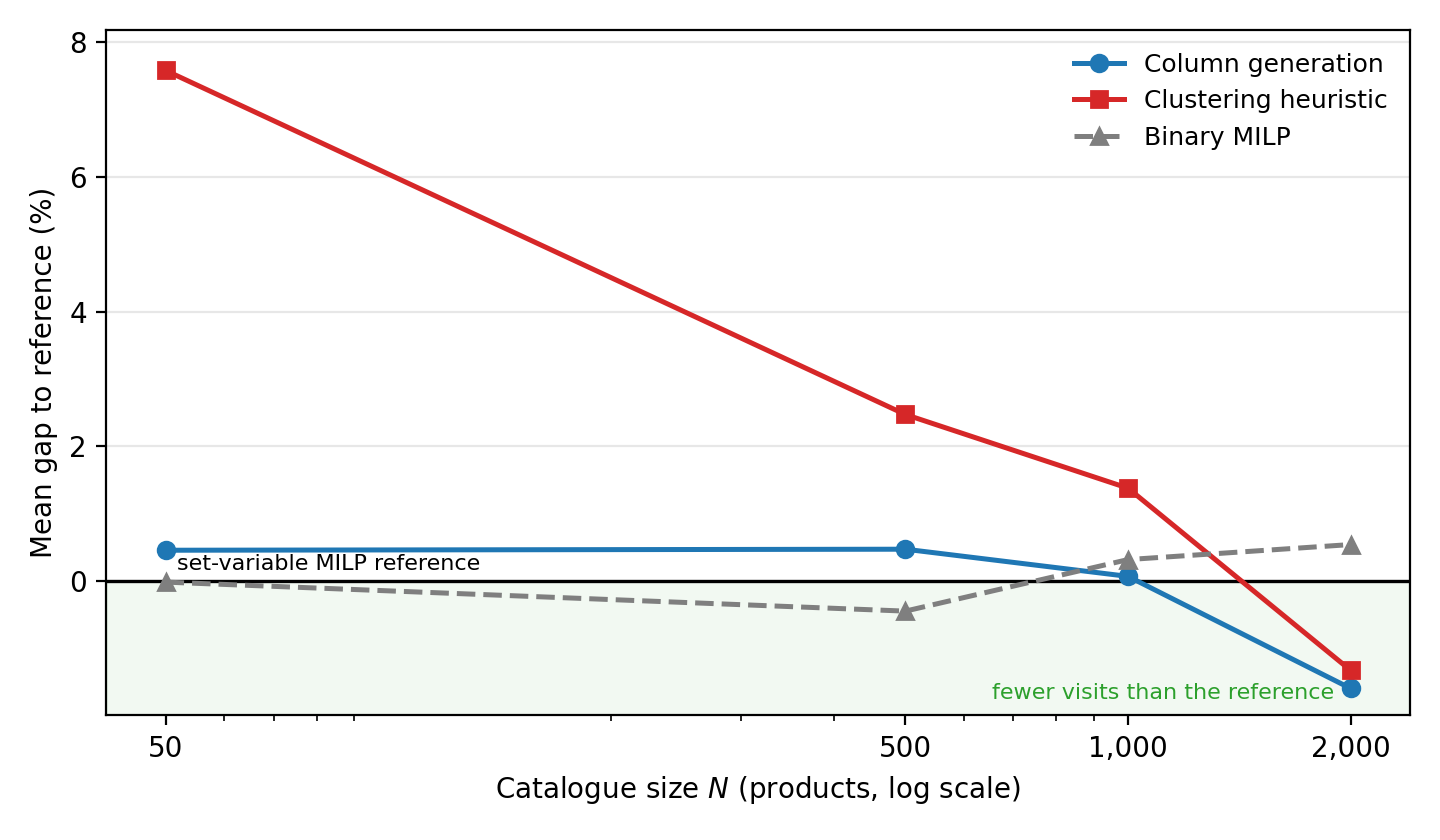
\includegraphics[width=0.86\linewidth]{Images_CSLAP/gap_vs_size_crossover.png}
\caption{Mean gap to the set-variable MILP reference against catalogue size. The reference is the horizontal line at zero, so a curve below it marks a method using fewer station visits. Both the column generation and the clustering heuristic cross the reference between 1,000 and 2,000 SKUs, ending $1.6\%$ and $1.3\%$ below it. The binary MILP moves the other way without doing so monotonically, sitting level with the reference at 50 SKUs and $0.4\%$ below it at 500 before rising to $0.3\%$ and $0.5\%$ above at the two larger sizes.}
\label{fig:crossover}
\end{figure}

\textbf{Both literature baselines trail, and the objective accounts for it.} Their gap to the reference widens with size, from a few percent at 50 SKUs to more than a quarter at 2,000, and neither returns fewer visits than the reference on a single instance at any of the four sizes. We attribute this primarily to the objective rather than to their tuning, though initialisation is also a factor, since the baselines start from their own prescribed initialisations (Section~\ref{sec:init}) whereas the optimising methods share the LPT start, and the two are not isolated experimentally here. The surrogate's dispersion term is directionally aligned with the visit objective, so it does not steer the search away from the metric on which the baselines are judged. What weakens with scale is the conversion rate between the two: swapping two products changes the visit count only when the swap removes an order's last product from a station or carries its first product to a new one, and most swaps do neither, so each generation or temperature level returns less as the catalogue grows. The LPT anchor is the opposite case, ignoring correlation altogether, so it spreads workload most evenly and pays the largest visit penalty at every scale.

\textbf{The heuristic's trade of quality for time does not merely improve with scale: it reverses.} It trails the search methods at 50 SKUs, closes to within a point and a half at 1,000, and at 2,000 returns fewer visits than the reference on all three instances in two minutes against twenty. The reason is the unit of work, the same mechanism the column generation exploits, and it is the composition of the move rather than its size that matters. The heuristic commits a whole community to a station in one step, and that community is assembled from products that are ordered together, so a single step can remove an order's last product from a station. The baselines also move groups, since the genetic algorithm's crossover copies a contiguous block of up to a quarter of the catalogue, but the block is drawn without reference to co-occurrence and then repaired for capacity, so it rearranges many products while rarely emptying a station of any order's products. A correlation-blind group move therefore buys no more of this objective than a single-product swap does, and its effort per product falls with scale where the heuristic's does not. Indexing the community bound on the station's slot capacity rather than on the catalogue (Section~\ref{sec:heuristic}) makes that unit grow with the station, which is what carries the effect to the largest size. From 500 SKUs upward it overtakes both literature baselines. The reversal at 2,000 SKUs rests on the same three instances as the crossing above, so we report it as an observed reversal on this benchmark rather than as a general catalogue size beyond which the heuristic leads. Where the column generation returns before its cap it does so because its generation loop is allotted a fraction of that cap and the closing stages finish inside theirs, not because it has priced out its master. It reached that generation limit on every instance at every size, so a longer budget could improve any of its rows.


% =====================================================================
\section{Industrial application}\label{sec:industrial}
% =====================================================================
We validate the framework on a real warehouse, Company~A, with $|P| = 21{,}874$ products and 26 stations, 24 of which carry movable SKUs after pruning and enter the solvers and the evaluation. The two static stations, S25 and S26, hold 1 and 2 locations and are not re-slotted between cycles. Products appearing in at most five orders and already held at a static station are frozen at their current location, leaving $15{,}975$ free to relocate and fixing the remaining $5{,}899$. Frozen products retain their slots and their share of station workload, so the solver receives the tolerance remaining after their load is accounted for, while the evaluation charges every station with its complete load on the complete order stream, and the reductions below are therefore not inflated by the reduced decision pool.

On this site the workload row \eqref{eq:wl} is applied per station in lines rather than in time. Each station's budget $T_s$ is set at $110\%$ of the lines its movable products carried under the legacy placement, which is \eqref{eq:wl} with $V_s$ normalised to that station's own calibrated speed, so a station is measured against the throughput it is engineered for and the cap is a line count for every station. Speeds and geometries differ across stations, so an absolute line count is not comparable between them. We therefore report each station's utilisation, its realised load as a percentage of its own full legacy load, and take the standard deviation of those percentages across the 24 evaluated stations. Because that denominator is the station's own legacy load, the legacy layout has zero dispersion on this measure by construction, so the metric reads as departure from the balance the site currently operates rather than as balance in the abstract.

\begin{table}[H]
\centering
\tbl{Industrial case study (Company~A, 24 evaluated stations) under a 10-hour cap. Green marks the best value in a column, orange the runner-up, red a workload violation; the shaded top row is the layout the site operates today.}
{\footnotesize\setlength{\tabcolsep}{3.5pt}\begin{tabular*}{\textwidth}{@{\extracolsep{\fill}}lrrrrrrr@{}}
\toprule
Method & Visits & Reduction (\%) & Gap vs.\ ref (\%) & Time (s) & Max WL & Util.\ SD (\%) & Viol. \\
\midrule
\rowcolor{yellow!50!black}
\textcolor{white}{Original layout (A)} & \textcolor{white}{1{,}062{,}507} & \textcolor{white}{--} & \textcolor{white}{15.81} & \textcolor{white}{0} & \textcolor{white}{9{,}923} & \cellcolor{green!80!black}\textcolor{white}{0.00} & \textcolor{white}{None} \\
Set-variable MILP & \textcolor{green!60!black}{\textbf{917{,}465}} & \textcolor{green!60!black}{\textbf{13.65}} & 0.00 & 36{,}000 & 10{,}467 & 4.48 & None \\
Binary MILP & \textcolor{orange!90!black}{\textbf{989{,}320}} & \textcolor{orange!90!black}{\textbf{6.89}} & 7.83 & 36{,}000 & 10{,}356 & \textcolor{orange!90!black}{\textbf{3.44}} & None \\
CG (station-indexed) & 1{,}000{,}844 & 5.80 & 9.09 & 36{,}000 & 10{,}074 & \textcolor{green!60!black}{\textbf{2.41}} & None \\
Heuristic & 1{,}044{,}932 & 1.65 & 13.89 & \cellcolor{blue!12}\textbf{647}\textsuperscript{$\dagger$} & 10{,}911 & 27.90 & None \\
GA & 1{,}046{,}071 & 1.55 & 14.02 & 19{,}358 & \textcolor{red}{\textbf{10{,}972}} & 18.52 & \textcolor{red}{\textbf{WL}} \\
SA-C & 1{,}058{,}563 & 0.37 & 15.38 & 36{,}000 & 10{,}811 & 12.14 & \textcolor{red}{\textbf{WL}} \\
\bottomrule
\end{tabular*}}
\tabnote{Reduction is against the original layout, Gap vs.\ ref against the set-variable MILP. Util.\ SD is the standard deviation of each station's realised load against its own legacy load (\%). Max WL is the realised busiest-station load in lines, the form of \eqref{eq:wl} used on this site. The site tolerates up to 10\% above the legacy load of the movable products a station holds, which is the same quantity the body uses throughout, and the busiest legacy station carries 9,923 lines, so its bound is 10,915. The flag marks a method whose realised load exceeds its own bound at one or more stations; the check is per station, so a breach can occur away from the busiest station, and a Max WL below 10,915 does not by itself certify feasibility. Time is the cap where a method exhausted its budget, otherwise the measured running time. \textsuperscript{$\dagger$}The heuristic's entry covers the whole $\beta$-selection search described in this section: seven layouts averaging 92 seconds each. The layout in this row is one of those seven. The heuristic remains the fastest method in the table; the next fastest takes about thirty times as long.}
\label{tab:industrial}
\end{table}

Table~\ref{tab:industrial} reports the outcome on the operating site, where the methods separate on feasibility before they separate on visits. The heuristic occupies the fast end of that separation, holding every station inside the site's tolerance (Figure~\ref{fig:workload}a) and still improving on the live layout. That improvement is the smallest of the feasible reductions, but it is the only one available at that running time, since the two metaheuristics take hours and still leave stations over their limits. It achieves that speed at a cost the visit column does not show: its utilisation dispersion is the highest in the table and the individual shifts span $[-83.8\%, +10.0\%]$, so while it respects every cap it fills some stations to the edge of the tolerance and leaves others far below their legacy load.

\textbf{The community bound does not transfer to this site, and the reason is instructive.} Section~\ref{sec:heuristic} sets $\beta$ from a single slot capacity, which presumes interchangeable stations. Here the stations hold between 8 and 2{,}575 movable products, and the rule applied to their mean returns $\beta=266$, which no repair can make feasible: a community sized for the average station cannot fit the small ones, so placement overloads them and the repair spends itself undoing placement rather than balancing it. Nor is the failure a matter of overshooting, because across the nineteen values of $\beta$ we evaluated feasibility is not an interval. Settings of $15$, $33$, $47$, $350$ and $450$ yield a feasible layout, whereas the other fourteen, spread from $63$ to $399$, do not. We can only offer a hypothesis for the two large feasible settings, which the data does not let us test: once $\beta$ passes the capacity of all but the largest stations, almost every community has to be split at placement, and the split rule that then governs the layout places products one at a time by the same admissibility test, so the blocks it produces are sized by what the stations can take rather than by $\beta$. On that reading the middle of the range is the worst place to sit, because communities are too large for the small stations and too small to force the split path throughout. We therefore select $\beta$ by evaluating a grid anchored on the mean capacity, $\{33,67,133,200,266,333,399\}$, and keeping the feasible layout with fewest visits. Exactly one of the seven is feasible, $\beta=33$, and it gives the heuristic row of Table~\ref{tab:industrial}, whose time entry charges the whole seven-point grid because that grid is the protocol a site would run. The other twelve settings were exploratory, and we exclude them from the reported cost for that reason rather than because they were cheap: charging all nineteen would raise the heuristic to roughly 1,750 seconds, still an order of magnitude below the next fastest method. Two of those exploratory settings are better and feasible, $\beta=350$ and $\beta=450$ at $1{,}030{,}978$ and $1{,}036{,}764$ visits, but no grid we could have specified in advance selects them, and we report them as a limitation rather than a result. On a warehouse of interchangeable stations none of this arises, the rule's $\beta$ being feasible on all 29 benchmark instances.

The set-variable MILP takes the opposite position, removing 13.7\% of the station visits while every station's utilisation shift stays within $[-5.9\%, +9.6\%]$, inside the site's 10\% slack (Figure~\ref{fig:workload}b), so the deepest reduction we obtain is also deployable. No method here returns a certified optimum, so this layout is the best found rather than a proven one. The binary MILP, given the same engine and budget, is also feasible at every station, yet carries 7.8\% more station visits, so with model, engine and budget identical the difference lies in the decision representation. At 21,874 products the $|P| \times |S|$ repair burden the set encoding removes is no longer negligible, and the synthetic family, where the two forms differ by less than 0.6\% at every scale (Section~\ref{sec:reliability}), gives no warning of it. A benchmark of a few thousand products would have retired the reformulation as redundant, which is why we retain it.

\begin{figure}[H]
\centering
\footnotesize
(a) Clustering heuristic\par\smallskip
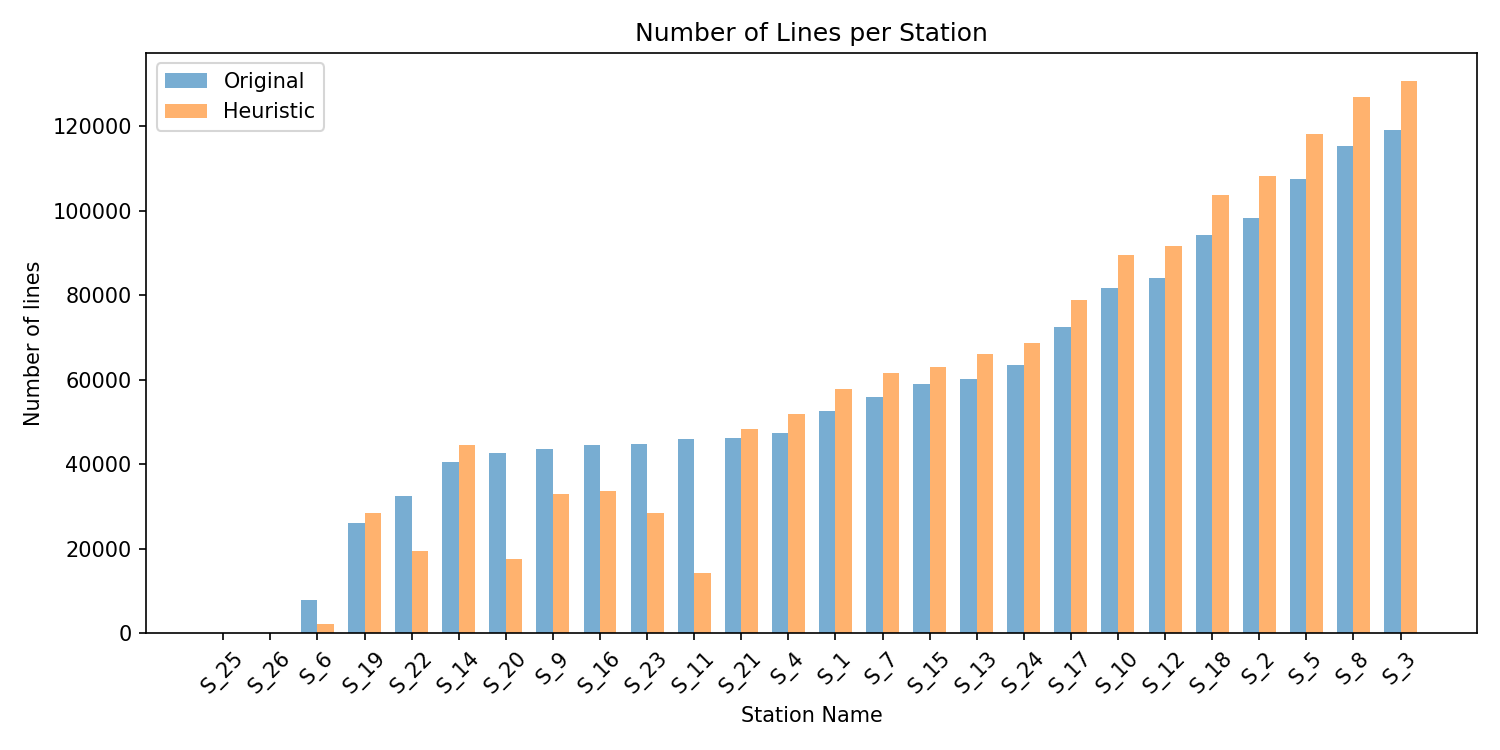
\includegraphics[width=0.46\linewidth]{Images_CSLAP/r4_number_of_lines_per_station.png}\hfill
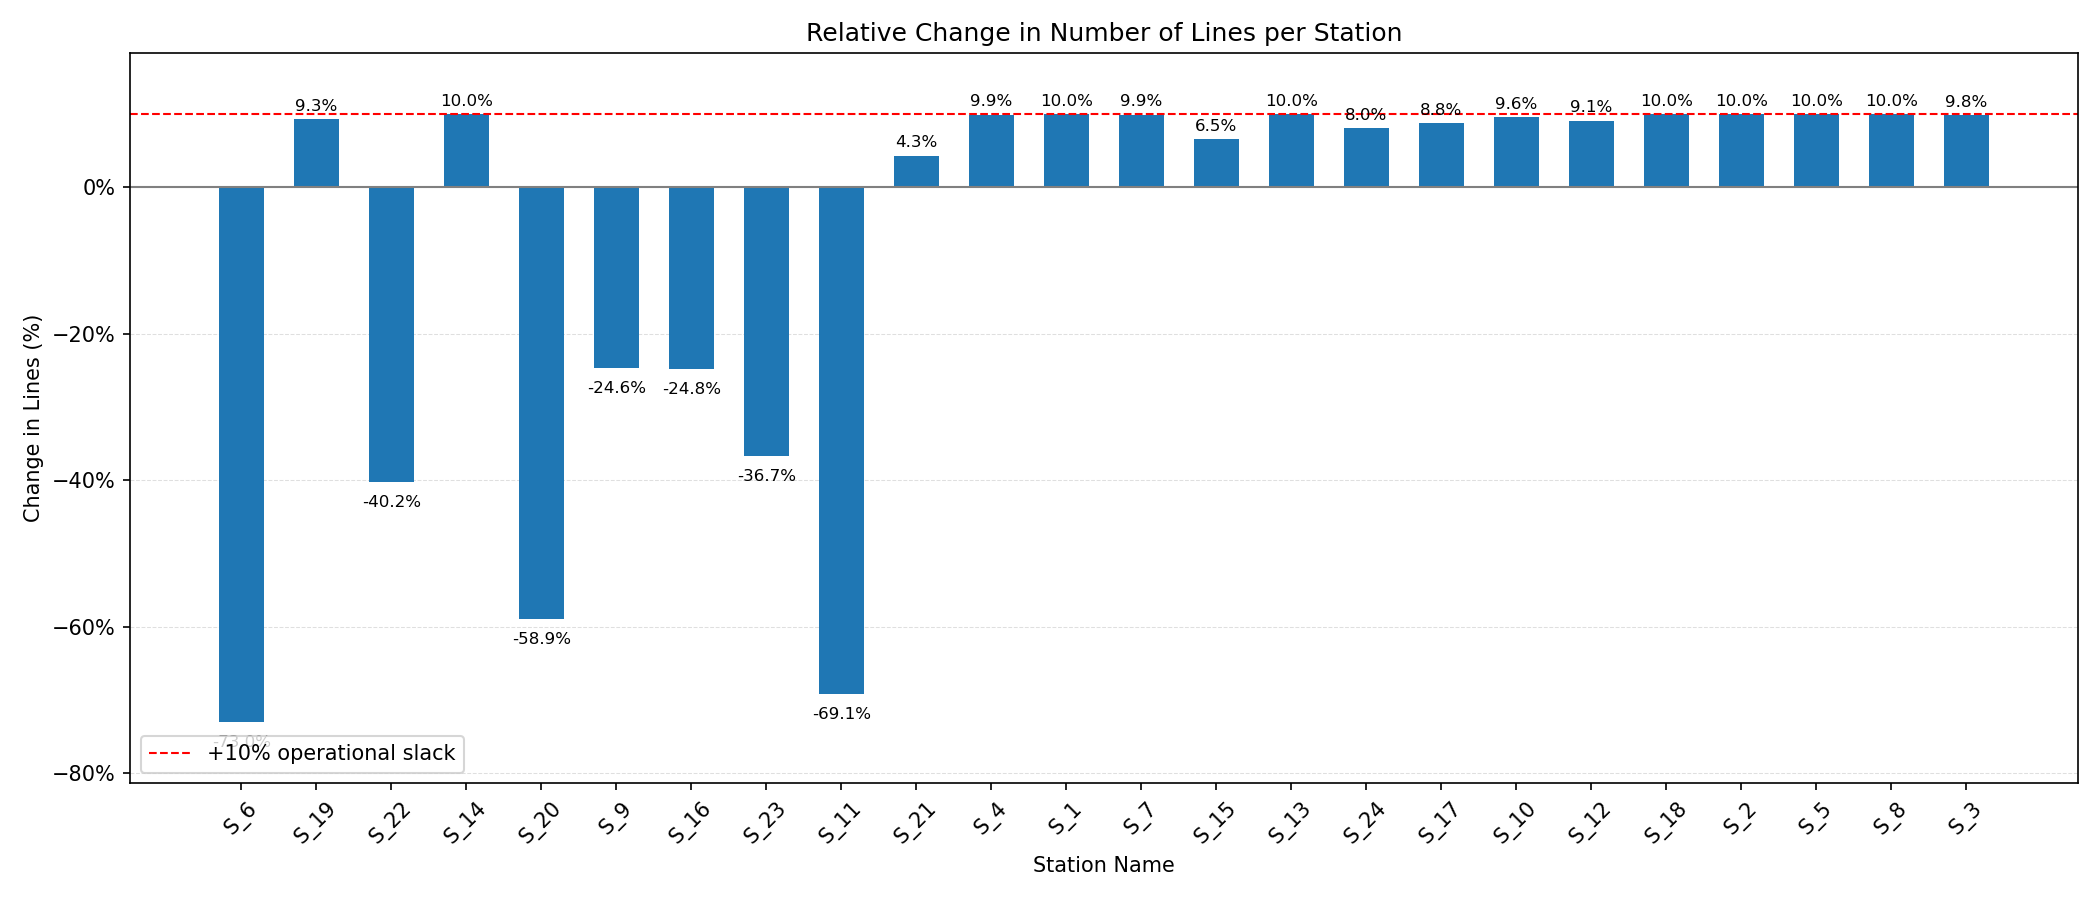
\includegraphics[width=0.46\linewidth]{Images_CSLAP/r5_pct_change_lines_per_station.png}\par\medskip
(b) Set-variable MILP\par\smallskip
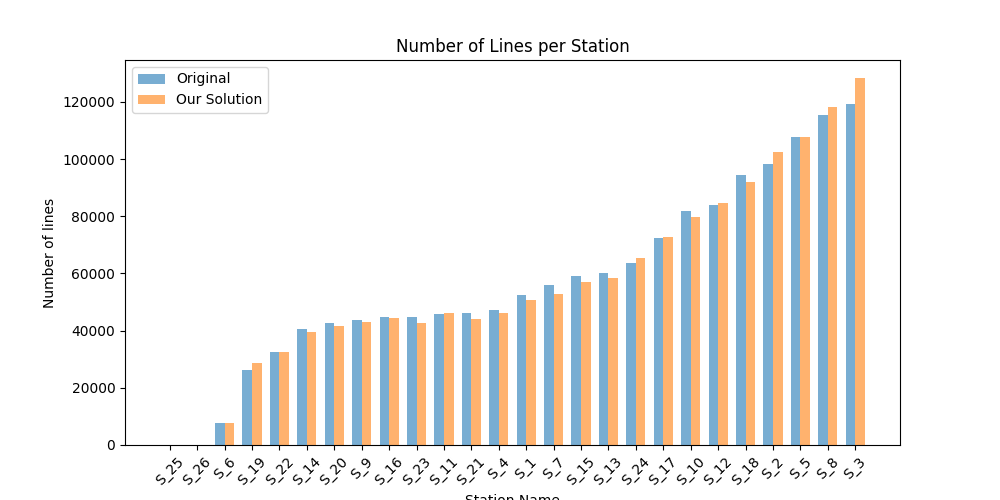
\includegraphics[width=0.46\linewidth]{Images_CSLAP/Hexaly_number_of_lines_per_station.png}\hfill
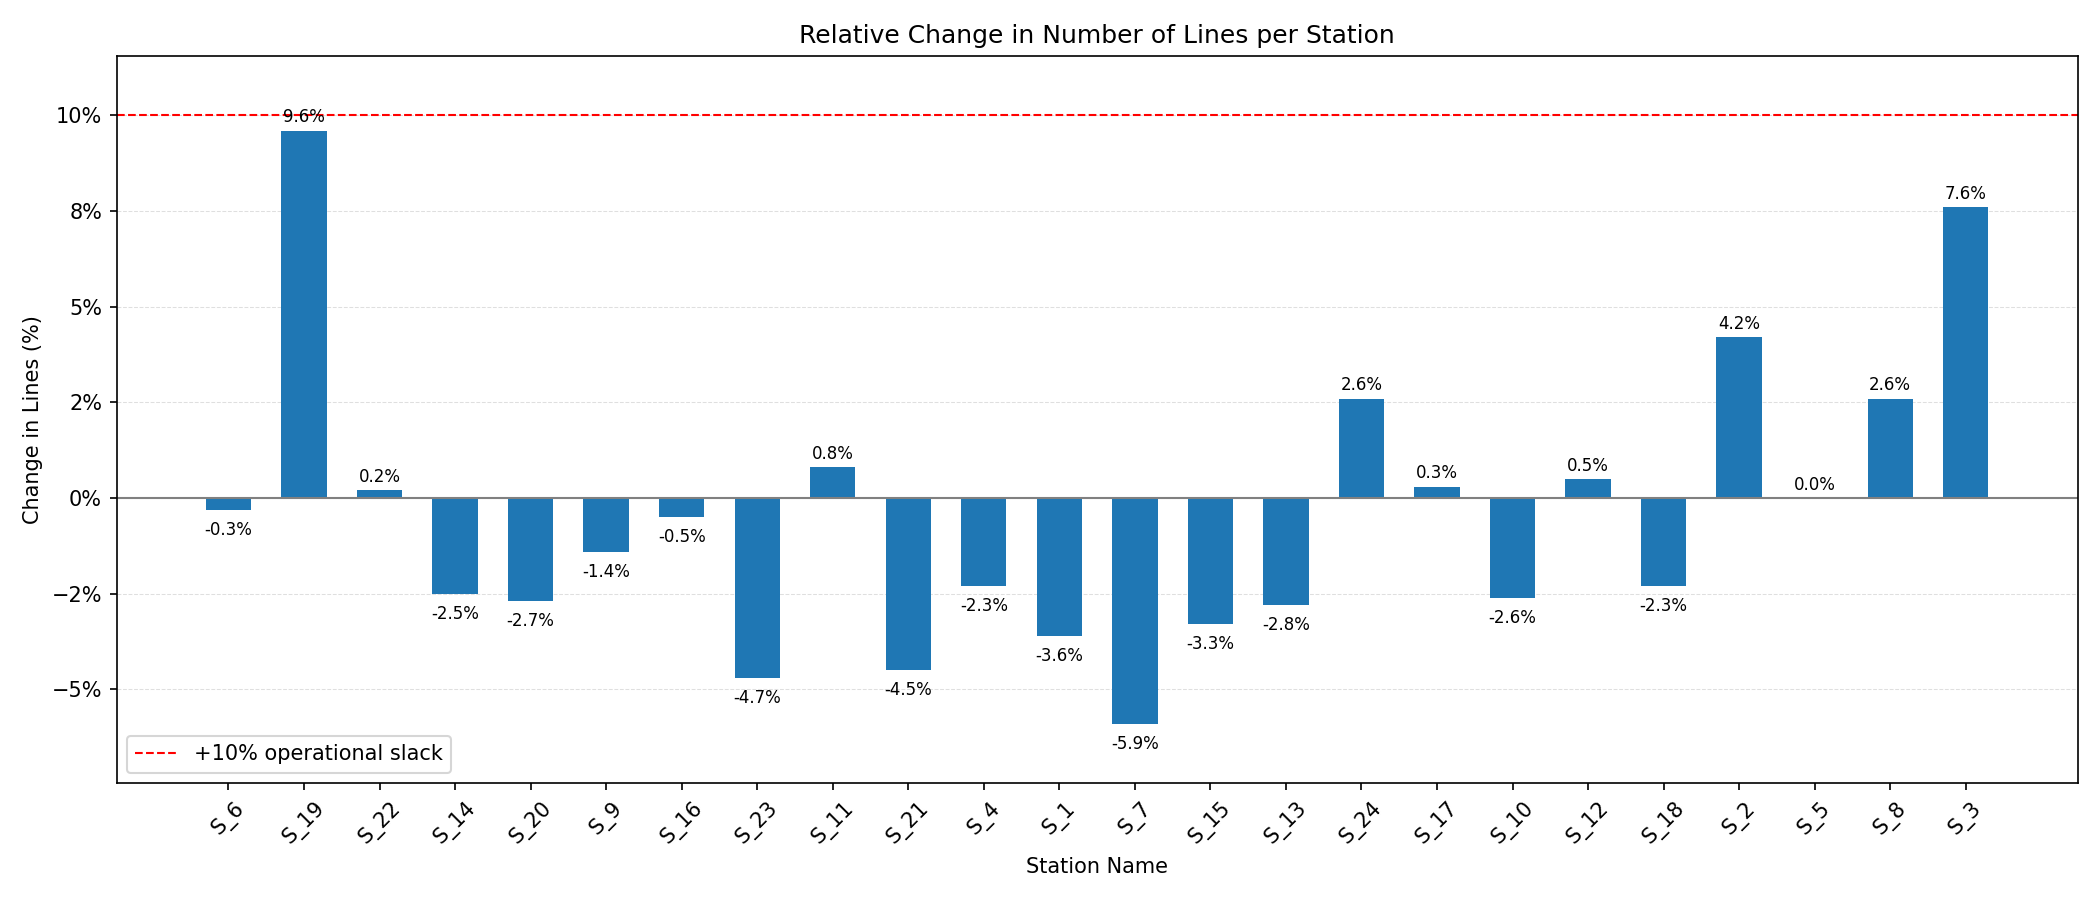
\includegraphics[width=0.46\linewidth]{Images_CSLAP/Hexaly_pt_relative_change_number_of_lines_per_station_new.png}\par\medskip
(c) Station-indexed column generation\par\smallskip
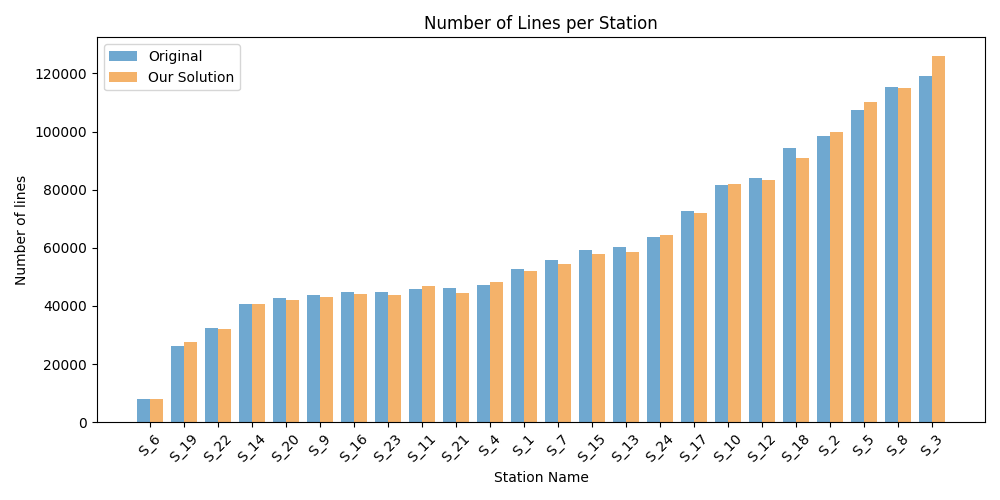
\includegraphics[width=0.46\linewidth]{Images_CSLAP/CG_SetPart_number_of_lines_per_station.png}\hfill
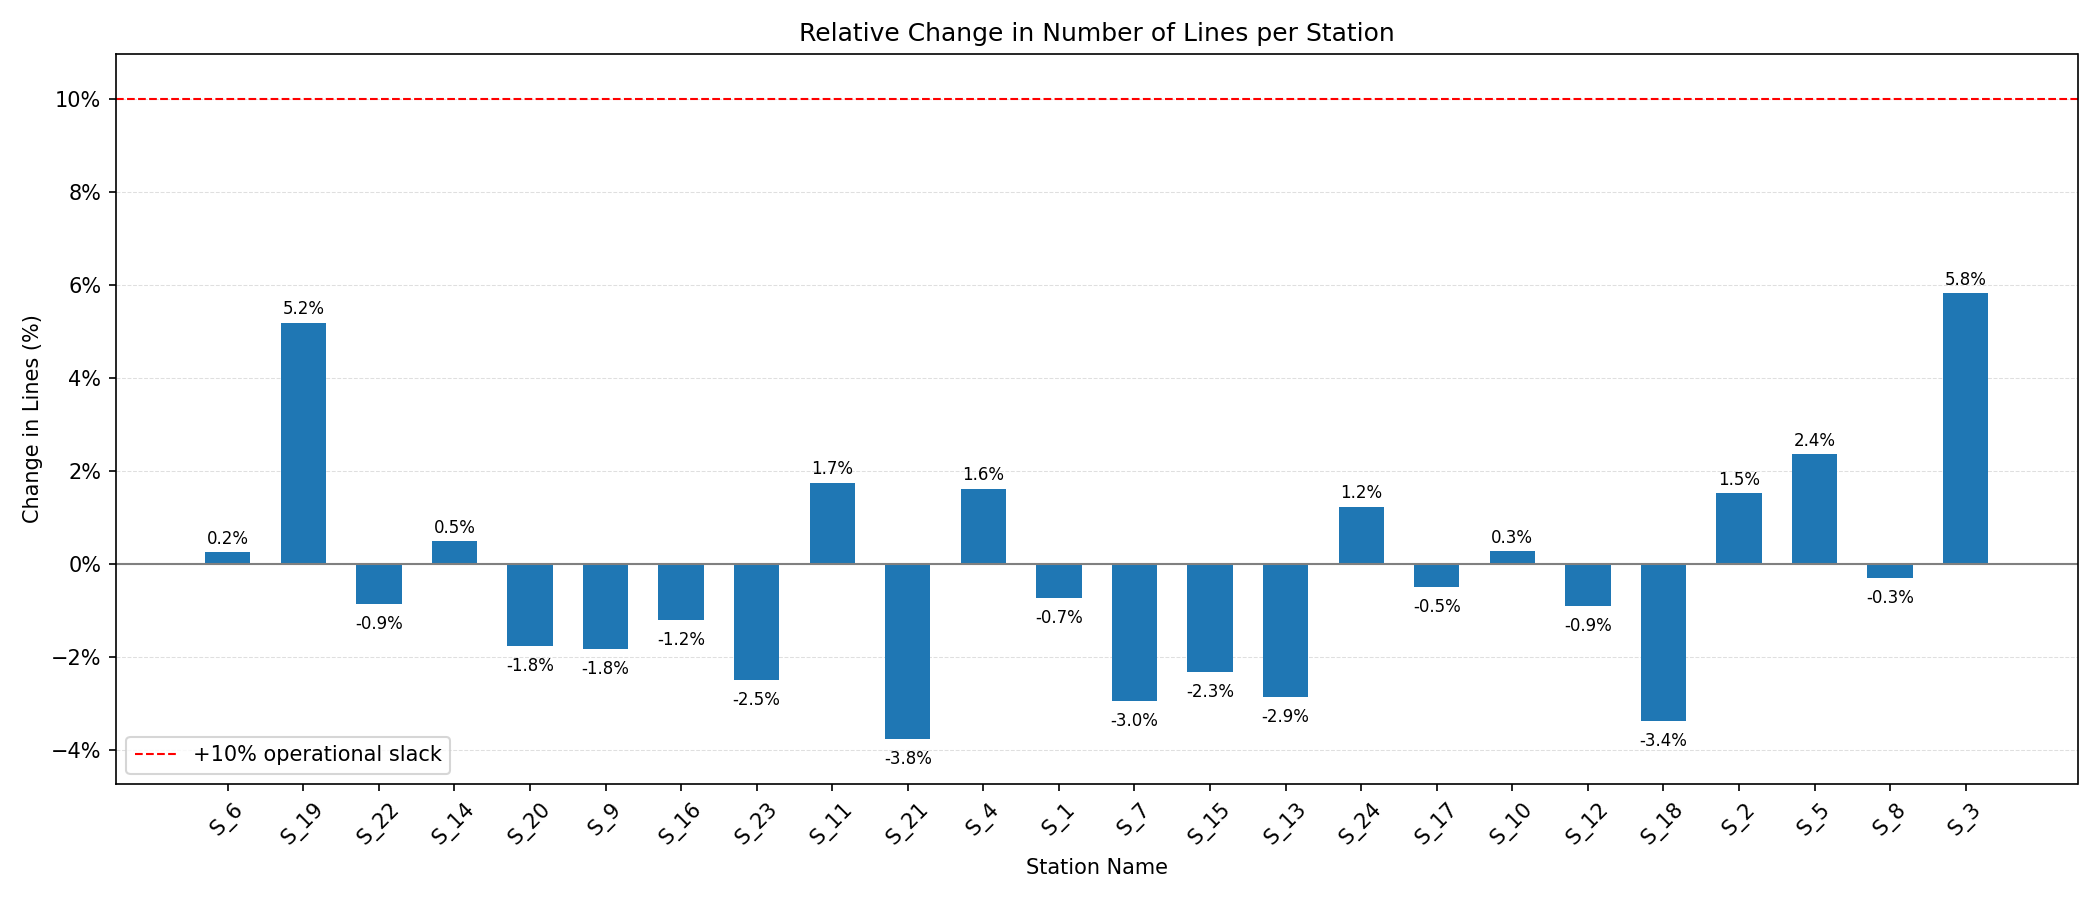
\includegraphics[width=0.46\linewidth]{Images_CSLAP/CG_SetPart_pt_relative_change_number_of_lines_per_station_new.png}
\caption{Station workload for the three deployable layouts against the original placement, with (a) the clustering heuristic, (b) the set-variable MILP and (c) the station-indexed column generation: lines per station (left) and relative change in utilisation (right). No station exceeds the site's $+10\%$ tolerance, and layout (c) tracks the engineered legacy balance most closely. The static stations S25 and S26 are omitted from the right-hand panels, where they would show 0\% by construction.}
\label{fig:workload}
\end{figure}

The column generation ran on Company~A in its station-indexed form with the set-variable MILP's inputs, so the two methods solve the same constrained problem. Each active station keeps its own convexity row, and the single persistent pricing model serves all of them by swapping the two station-dependent right-hand sides per call. Two elements differ from the homogeneous drive. The warm start is the live layout rather than an LPT partition, so the run improves the operating configuration step by step, and priced bundles are installed by an ejection-style recompletion that evicts the bundle's products, rebuilds the target station and reinserts the displaced products by co-occurrence affinity, instead of rebuilding a partition from scratch. The run priced exactly throughout and used its full cap, removing 5.8\% of the visits the site incurs today.

That shallower reduction is obtained with a smaller disturbance to the existing balance. The column-generation layout has the same feasibility profile as the set-variable solution, both exceeding the raw legacy load on ten stations and both remaining inside the site's 10\% tolerance everywhere, yet its utilisation dispersion is the lowest of any optimising method in Table~\ref{tab:industrial} (Figure~\ref{fig:workload}b, c), which under the legacy-anchored definition means it departs least from the distribution of work the site currently operates. The drive produces that profile: warm-starting from the live layout and installing one priced bundle at a time keeps it near the incumbent balance, and enforcing the workload cap inside pricing means no violating bundle is ever generated. The Farley pass ran to completion but stays uninformative at this scale, consistent with Section~\ref{sec:cgbound}. The site therefore has two deployment profiles, the set-variable MILP for the deepest visit reduction and the column generation when the objective is an improvement that barely moves the engineered balance.

The site runs about 81,700 station stops a week across the extract. A planning figure has to be built on the reduction the layout holds on weeks it was not fitted to, which Section~\ref{sec:temporal} puts at 6.6 to 7.4\%, so the expected saving is roughly 5,400 to 6,050 fewer stops per week. The in-sample 13.7\% would give about 11,150, and we quote it only as the ceiling reached if demand does not move. Each eliminated visit removes one cycle of deceleration, induction, scanning and merge. That cycle time is site-specific and we do not measure it, so we state the effect per unit: for every second of per-visit cycle time the out-of-sample reduction frees between 1.5 and 1.7 hours of station dwell per week, against 3.1 hours at the in-sample rate. The projection is linear and ignores queueing, so a discrete-event study is needed to confirm it (Section~\ref{sec:perspectives}).

\subsection{Robustness on unseen weeks}\label{sec:temporal}
A layout is optimised once and then operated as demand evolves, so we test out of sample. The dataset spans 13 weeks, from 1 September to 30 November 2021, and the splits are cut on the recorded delivery date of each order: the model sees the first 10 weeks and is evaluated on the last 3, then sees the first 8 and is evaluated on the last 5. Each layout is compared with the original placement and with an oracle optimised directly on the test weeks, following robustness practice in storage assignment \citep{lee2020cie, wang2020}.

This test separates two quantities the paper must not conflate. The 13.7\% of Table~\ref{tab:industrial} is an in-sample figure: the layout was optimised on the same 13 weeks it is then measured over. On weeks the model never saw, the same method removes 6.6\% of visits on the three-week hold-out and 7.4\% on the five-week one (Table~\ref{tab:temporal}). The deployable expectation for a site re-slotting on recent history is therefore the second pair, with the first standing as an upper bound reached only when demand does not move. The gap is not solver quality. An oracle optimised directly on the test weeks removes 12.1\% and 10.2\% there, so most of what separates 13.7\% from 6.6\% is demand drift rather than anything the method failed to find.

Read against that oracle, the fitted layouts retain 55\% of the available reduction on the three-week hold-out and 72\% on the five-week one. The share rises with the evaluation window, consistent with the oracle's advantage being concentrated in short-lived demand patterns that a longer window averages out, though the two splits vary the training and evaluation windows together, so the effect of each is not separated here. Recent history is therefore sufficient for a durable gain on this site, though that stability may not carry to more volatile assortments.

\begin{table}[H]
\centering
\tbl{Out-of-sample station-visit performance on held-out weeks.}
{\begin{tabular*}{\textwidth}{@{\extracolsep{\fill}}llrrr@{}}
\toprule
Test period & Layout (training period) & Total visits & Mean visits & Reduction (\%) \\
\midrule
\multirow{3}{*}{Last 3 weeks}
 & Original placement & 265{,}876 & 4.052 & -- \\
 & Optimised on first 10 weeks & 248{,}358 & 3.785 & 6.6 \\
 & Oracle (optimised on last 3 weeks) & 233{,}728 & 3.562 & 12.1 \\
\midrule
\multirow{3}{*}{Last 5 weeks}
 & Original placement & 423{,}593 & 3.926 & -- \\
 & Optimised on first 8 weeks & 392{,}318 & 3.636 & 7.4 \\
 & Oracle (optimised on last 5 weeks) & 380{,}356 & 3.525 & 10.2 \\
\bottomrule
\end{tabular*}}
\tabnote{All layouts are produced by the set-variable MILP under the 10-hour cap of Table~\ref{tab:industrial}, the training window being the only thing that changes. Mean visits is total visits divided by the number of orders in the test period, that is the average number of stations an order visits. Reduction is against the original placement on the same test window, so it is measured out of sample for the fitted layouts and in sample for the oracle.}
\label{tab:temporal}
\end{table}

\subsection{Bounded reassignment}\label{sec:reassign}
An established facility cannot absorb a disruptive re-slotting wave \citep{chabot2024reassignment}, so we bound how many products may move. With $s'(p)$ the legacy station of product $p$, the single constraint
\begin{equation}
\sum_{p \in P} x_{p,\,s'(p)} \ \ge\ |P| - k
\label{eq:reassign}
\end{equation}
limits the number of relocated products to at most $k$. Nothing else changes, and the legacy layout stays feasible for every $k$, so the model has a solution whatever budget the site sets. We solve it with the set-variable MILP for $k \in \{250, 500, 1000, 2000, 5000\}$ under a one-hour limit each, against the legacy layout ($k=0$) and the full re-optimisation (Table~\ref{tab:reassign}, Figure~\ref{fig:ksweep}). The same limit fits the column-generation framework, where counting for each bundle how many of its products would leave their legacy station turns \eqref{eq:reassign} into one knapsack-style row whose dual enters pricing as a per-product relocation penalty. We have not run that variant.

\begin{table}[H]
\centering
\tbl{Bounded-reassignment trade-off on the industrial instance.}
{\small\begin{tabular*}{\textwidth}{@{\extracolsep{\fill}}lrrrrr@{}}
\toprule
Relocation cap & \% catalogue & Total visits & Reduction & \% of full benefit & WL-viol.\ stations \\
\midrule
Legacy ($k=0$) & 0\% & 1{,}062{,}507 & -- & -- & 0 \\
$k=250$        & 1.1\% & 1{,}061{,}302 & 1{,}205 & 0.8\% & 0 \\
$k=500$        & 2.3\% & 1{,}060{,}120 & 2{,}387 & 1.6\% & 0 \\
$k=1{,}000$    & 4.6\% & 1{,}056{,}412 & 6{,}095 & 4.2\% & 0 \\
$k=2{,}000$    & 9.1\% & 1{,}049{,}730 & 12{,}777 & 8.8\% & 0 \\
$k=5{,}000$    & 22.9\% & 1{,}034{,}735 & 27{,}772 & 19.2\% & 0 \\
Full re-opt.   & --     & 917{,}465 & 145{,}042 & 100\% & 0 \\
\bottomrule
\end{tabular*}}
\tabnote{``\% catalogue'' is $k$ as a share of all 21,874 products; only the 15,975 movable ones can relocate. ``\% of full benefit'' is the reduction as a share of the 145,042 visits removed by the full re-optimisation.}
\label{tab:reassign}
\end{table}

\begin{figure}[H]
\centering
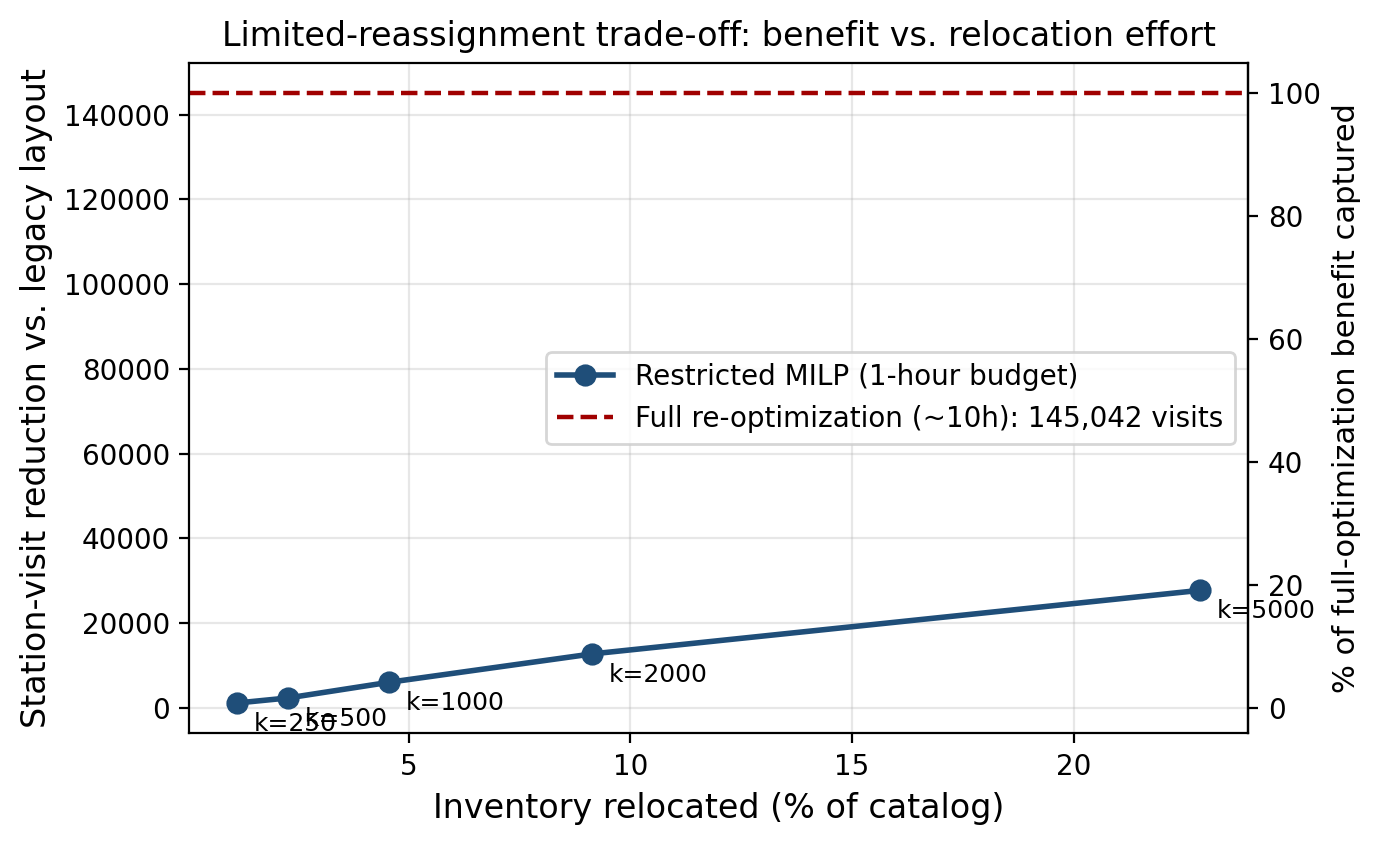
\includegraphics[width=0.7\linewidth]{Images_CSLAP/reassignment_ksweep_curve.png}
\caption{Station-visit reduction against the share of the catalogue relocated. The dashed line marks the reduction achieved by the full re-optimisation.}
\label{fig:ksweep}
\end{figure}

Bounded re-slotting returns benefit sub-proportionally to effort at every cap we sample, the share of the full reduction captured staying below the share of relocatable stock actually moved: at $k = 5{,}000$, which is $31.3\%$ of the $15{,}975$ movable products, the layout captures $19.2\%$ of the available reduction. The curve shows no inflection point at which a small subset of moves captures a disproportionate share of the gain. Per relocated product a bounded budget also returns less than a full rearrangement: the first 5,000 relocations return about 5.6 visits each, whereas the full re-optimisation returns at least $145{,}042/15{,}975 \approx 9.1$ even on the conservative assumption that it moves every movable SKU\@. The bounded runs are given one hour each against the ten hours of the full re-optimisation, but the shortfall is far larger than a longer search would close and grows with the tightness of the cap rather than with the time available. The objective explains the asymmetry. A visit disappears only when an order loses its last product at a station, so relocating part of a co-ordered group yields no reduction until the remainder follows, and consolidation realised only in whole groups means a partial budget cannot obtain a proportional share of it.

The curve is nonetheless the quantity a manager requires, because every point on it is deployable: at each cap the solver keeps all stations within capacity and workload, and we verified separately that the busiest station load and the spread of utilisation stay close to their legacy values throughout. The relocation budget can therefore be set against available labour with a known marginal benefit rather than guessed. A site unable to absorb a full rearrangement in one cycle can plan successive bounded waves, each re-solved from the layout then in place, though how much of the full benefit such a sequence recovers is not something we measure.

% =====================================================================
\section{Managerial insights}\label{sec:managerial}
% =====================================================================
The results yield five implications for warehouse operations.

Track station visits as a slotting indicator. Each diversion generates mechanical queueing and handling delay, so stops per order expose congestion that a distance metric hides.

Read the labour effect as a planning figure, not a saving, and build it on the out-of-sample reduction. A layout measured on the weeks it was fitted to removes 13.7\% of visits, but on weeks it has not seen the figure is 6.6 to 7.4\% (Section~\ref{sec:temporal}), and only the latter describes what a site will operate with. The freed station dwell then scales with a site's own per-visit cycle time (Section~\ref{sec:industrial}), and the projection assumes that time is fixed and no queue forms, so a site should substitute its measured cycle time and commission a discrete-event study before treating the figure as realised.

Match the tool to the decision, and to the warehouse. Where stations differ in geometry and speed, as Company~A's do, the set-variable MILP gives the best layout we obtain within capacity. Where they are interchangeable, the choice shifts with catalogue size, and Section~\ref{sec:reliability} shows the ranking reversing between 1,000 and 2,000 SKUs on this benchmark without fixing the size at which it turns. Where the priority is minimal disturbance to an engineered balance, choose the column generation, which held the workload limit in every experiment. The clustering heuristic is the choice where a layout is needed quickly or often, and on a large catalogue of interchangeable stations it is no longer only that, returning fewer visits than either MILP representation at 2,000 SKUs in two minutes rather than twenty. Two conditions attach. It disturbs the existing distribution of work the most, so a site adopting it should check station-level loads against its own operational tolerance and not against the cap alone, and its community bound presumes stations that are alike. Where they are not, Section~\ref{sec:industrial} shows the bound has to be searched for rather than computed, and the gain shrinks accordingly.

Improve continuously without a shutdown. The bounded-reassignment model lets a site move only as many products as its workforce can handle in one cycle, and every point on the curve of Table~\ref{tab:reassign} holds all stations within capacity and workload. Later waves should return more per relocated product than the first, since consolidation is realised in whole groups, though we do not measure a full sequence.

Recalibrate on a rolling window. A layout optimised on the most recent 8 to 10 weeks retains most of the reduction an oracle could obtain on the following weeks, so re-optimising at that cadence keeps the layout current for limited effort while the reassignment cap keeps each cycle non-disruptive.

% =====================================================================
\section{Research perspectives}\label{sec:perspectives}
% =====================================================================
Four tracks extend this work. Two concern the method. Dual stabilisation, for instance the boxed dual penalties of \citet{dumerle1999stabilized} or the weighted dual centres of \citet{wentges1997weighted}, is the first lever, and Section~\ref{sec:cgbound} gives the measured reason for choosing it over a stronger formulation: the master never priced out inside the cap on any instance, so the bound is limited by how far the dual iteration got rather than by the strength of the relaxation it converges to. Reaching $z_{\mathrm{LP}}$ within the budget would turn the metaheuristic reading into certified gaps, and only then would the residual distance be an integrality gap for a branch-and-price layer over the price-and-complete drive to close, while on the industrial side a longer horizon or a hybrid of the swap descent with the set-variable MILP would narrow the gap the station-indexed run leaves. A fuller experimental account of the drive would follow, isolating the contribution of the dual-guided greedy step, the completion policy and the final descent by controlled ablation, and carrying an adaptive large neighbourhood search and an open-source constraint-programming model \citep{ropke2006alns, perron2023cpsat} as additional baselines. Neither appears here, and Hexaly, whose search is itself neighbourhood-based, already occupies part of that design space, so the comparison we lack is chiefly what the approach costs a practitioner without a commercial licence.

Two concern the model. The first is product geometry: replacing the unit count of a station's capacity with a per-product footprint $f_p$ in \eqref{eq:cap}, coupled to the budget \eqref{eq:wl}, would admit three-dimensional packing limits without changing the structure of the programme, and the same extension covers duplicating a high-demand product across stations, which the single-station assumption currently excludes. In the decomposition that change is contained, since the covering rows \eqref{eq:cover} already allow a product in several bundles, so only the equality tying each product to one station has to be relaxed, with the replenishment cost of each extra copy charged in the pattern cost so pricing proposes a duplicate only when the visits it saves outweigh it. The second is the visit-to-throughput link. We balance workload, which lowers expected queueing, but do not model the queue, and feeding the optimised layouts into a discrete-event simulation would convert the planning figures of Section~\ref{sec:managerial} into measured throughput and open the way to stochastic demand and real-time routing.

% =====================================================================
\section{Conclusion}\label{sec:conclusion}
% =====================================================================
We posed the correlated storage location assignment problem for automated pick-and-pass warehouses with station visits as the objective and hard capacity and workload limits. The objective is piecewise constant, so it stalls branch-and-bound and metaheuristic search at scale, and two routes clear that barrier. A set-variable MILP produces feasible layouts that beat the literature baselines by a margin widening with size and lowers station visits on a real 21,874-product warehouse by 13.7\% while keeping every station within capacity, where the binary form of the same model carries 7.8\% more visits and so shows that the reformulation earns its place at scale. A set-partitioning column generation, driven as a price-and-complete metaheuristic, matches that reference at 1,000 products and leads at 2,000, never breaches a workload cap, carries a valid but loose lower bound, and on the industrial site improves the live layout by 5.8\% while disturbing the engineered balance least.

The clustering heuristic provides a fast fallback when tight computational budgets prevent exact or decomposition runs. Indexing its community bound on the slot capacity of a station rather than on the length of the catalogue, a choice we justify on a family of instances built to separate the two, carries it below the set-variable reference at 2,000 products in two minutes against twenty. That rule presumes interchangeable stations and does not hold on the industrial site (Section~\ref{sec:industrial}), where the bound has to be selected by search and the resulting layout departs furthest from the site's existing distribution of work. A bounded-reassignment extension maps the trade-off between re-slotting effort and benefit, making the gains deployable on an active site without a shutdown. What these layouts are worth in throughput rather than stops is the question we leave open, and answering it calls for the queueing model Section~\ref{sec:perspectives} sets out.

% ---------------------------------------------------------------------
% BACK MATTER (IJPR order)
% ---------------------------------------------------------------------
\section*{Author contributions}
All authors were involved in the conception, design and modelling of the framework. Ermal Belul developed the software, analysed the empirical data and drafted the manuscript; Marwane Bouznif, Dritan Nace and Antoine Jouglet critically revised it for intellectual content. All authors approved the final version and agree to be accountable for all aspects of the work.

\section*{Acknowledgements}
The authors thank the operational teams at Company~A for the dataset and for their insight into the picking process, and Savoye and the Universit\'{e} de technologie de Compi\`{e}gne for hosting the work.

\section*{Funding details}
This work was supported by the Association Nationale de la Recherche et de la Technologie (ANRT) under a CIFRE doctoral grant in partnership with Savoye.

\section*{Disclosure statement}
The authors report there are no competing interests to declare.

\section*{Declaration of generative AI use}
During the preparation of this work the authors used a generative AI assistant to refine language and improve readability. After using this tool the authors reviewed and edited the content as needed and take full responsibility for the content of the published article.

\section*{Data availability statement}
This journal applies the Taylor \& Francis ``share upon reasonable request'' data sharing policy. Both synthetic instance families are \href{https://anonymous.4open.science/r/Anonymized_Export_CSLAP_v2-01BC/README.md}{openly available online}, the 29 benchmark instances of Section~\ref{sec:experiments} and the 80 calibration instances of the supplementary material, each with the generator, the station counts and the seeds that produced them. The same archive carries the per-instance convergence record behind Section~\ref{sec:cgbound}, giving the convergence status, $z_{\mathrm{RMP}}$, $\mathrm{rc}_{\mathrm{lb}}$ and the generation-loop deadline for every column-generation run. The de-anonymised permanent link will be provided on acceptance. The Company~A dataset cannot be made public because of commercial confidentiality, and may be requested from the authors under reasonable operational conditions, as may the dated extract behind Table~\ref{tab:temporal}. The solvers, Hexaly and IBM CPLEX, depend on commercial licences we cannot redistribute, and the model statements and settings needed to rebuild the methods on another solver are given in Sections~\ref{sec:model}, \ref{sec:cg} and~\ref{sec:experiments}.


% ---------------------------------------------------------------------
% References (APA via apacite)
% ---------------------------------------------------------------------
\bibliographystyle{apacite}
\bibliography{IJPR_CSLAP}

% ---------------------------------------------------------------------
% APPENDIX
% ---------------------------------------------------------------------
\appendix
\section{Implementation details and baseline configurations}\label{app:impl}
\subsection{Incremental evaluation of the swap descent}\label{app:swapeval}
The descent of Section~\ref{sec:cgdrive} keeps a support-count matrix $\mathrm{cnt}[i][u]$, the number of products of station $i$ contained in support $u$. Station $i$ visits $u$ exactly when $\mathrm{cnt}[i][u]>0$. Removing a product frees the supports whose count falls to zero and inserting it costs those whose count rises from zero. Only supports containing the two moved products can change, so a swap is scored in time proportional to their support degrees rather than by re-scanning the orders, and the counts are updated the same way once a swap is accepted.

\subsection{Solver budgets and baseline parameters}\label{app:baselines}
The time cap $B$ of Section~\ref{sec:cgdrive} is divided across the four stages. On the homogeneous benchmarks the warm start ends at $0.08B$, the generation loop at $0.70B$, the integer master at $0.85B$, and the final polish takes the remainder. The heterogeneous industrial run uses a schedule matched to its longer runs: warm start $0.05B$, generation loop $0.62B$, a bound pass at $0.74B$, integer master $0.82B$, and a closing polish.

Both baselines score a candidate layout with the same surrogate: the station-visit count, plus 1{,}000 times the total excess over slot capacity or workload cap, plus 0.01 times the co-occurrence weight of product pairs placed at different stations. The first term is the real objective, the second makes an infeasible layout uncompetitive, and the third breaks ties between layouts the visit count cannot separate.

The genetic algorithm carries 50 assignment vectors for at most 200 generations or until the per-size cap of Section~\ref{sec:experiments} is reached, with binary-tournament parent selection, crossover at probability 0.8 copying a contiguous segment of one parent into the other up to a quarter of the catalogue with a repair pass for over-capacity stations, mutation at probability 0.1 exchanging two products' stations, and the best layout of each generation carried forward unchanged. Each of the 50 initial members is drawn by assigning products to stations uniformly at random subject to $\zeta_s$, as \citet{pan2015} prescribe.

Simulated annealing with correlated interchange starts at temperature 800 and cools geometrically by 0.95 per level until the temperature reaches 1 or the cap is met, proposing $\min(2|P|, 1000)$ moves per level. A move is drawn from the correlated pair list, co-occurring pairs being sorted by descending co-occurrence and split into ten equal groups from which a group and then a pair are drawn uniformly, and the two products exchange stations. A move lowering the surrogate is always accepted, whereas one raising it by $\Delta$ is accepted with probability $\exp(-\Delta/T)$. The run starts from a cube-per-order-index (COI) layout, which is correlation-blind like LPT but ranks products by demand volume per unit of storage occupied rather than by order-line frequency, filling stations in that order \citep{kim2012}.

Every run reported in this paper was produced on the same remote machine, a 16-core Windows Server 2019 host with 128\,GB of memory, under the same Python 3.10 environment, and every method received the same core and thread allocation, four threads, so no method was given more compute than another under the shared wall-clock cap. The column generation runs on CPLEX 22.1.1 and the two MILP representations on Hexaly 13.0. One run per instance is reported in every cell. The two baselines are our own Python implementations of the published operators, so a residual implementation-efficiency difference against the two commercial engines cannot be excluded, and we record how far each baseline got rather than assume it exhausted its search.

Both metaheuristic baselines draw their search decisions from a NumPy generator seeded at 42, so SA-C is fully determined by the instance and the cap. The genetic algorithm's capacity repair draws instead on the global random stream, seeded at 20240612 by the experiment harness, and that stream is the only source of run-to-run variation in the reported GA figures. The column-generation drive is also stochastic, since Stage 1 mutates the warm start and the descent samples candidate partners beyond about 300 products, and it draws on the same harness stream. We report one run per cell for it as well, so the 2,000-SKU result rests on three single draws and a replicated cell would strengthen it.

\section{Mathematical proofs of bounding claims}\label{app:bounds}

\subsection{Binary MILP linear relaxation floor}\label{app:bounds_milp} Take any point satisfying $\sum_{s\in S} x_{ps}=1$. For an order $o \in O$ and a product $p \in P_o$, the linking row $x_{ps}\le z_{os}$ forces $z_{os}\ge x_{ps}$ for every station, and summing over the stations gives $\sum_{s\in S} z_{os}\ge\sum_{s\in S} x_{ps}=1$. The objective therefore cannot fall below $|O|$ at any feasible point, fractional or integral. That floor is attained: setting $x_{ps}=1/|S|$ meets the capacity rows whenever $|P|/|S|\le\zeta_s$ and the workload rows under the operational slack of Section~\ref{sec:experiments}, so $z_{os}=1/|S|$ is feasible and the objective equals $|O|$ exactly. On this instance family the relaxation is therefore worth precisely the statement that every order visits at least one station, independent of the co-occurrence structure that makes one instance harder than another, so a branch-and-bound search starts from that value with nothing instance-specific to prune with.

\subsection{Column generation Farley-type dual bound}\label{app:bounds_cg} The bound does not rest on the price-and-complete drive. It follows from linear-programming duality applied to the restricted master together with a valid dual bound from the pricing solve, and would hold whatever heuristic produced the layouts.

Write the restricted master of Section~\ref{sec:cgagg} with duals $\sigma_p\ge 0$ on the covering rows and $\mu\le 0$ on the cardinality row. The upper bounds $y_q\le 1$ may be dropped, since reducing any $y_q$ above one to one preserves coverage, relaxes the cardinality row and cannot increase the objective, so an optimal dual solution with zero multipliers on them exists. Strong duality gives $z_{\mathrm{RMP}}=\sum_p\sigma_p+|S|\mu$. The pair $(\sigma,\mu)$ need not be dual-feasible for the full master, because a bundle outside the pool may price out negatively. Let $\mathrm{rc}_{\min}$ be the least reduced cost over all feasible bundles and suppose it is negative. Replacing $\mu$ by $\mu'=\mu+\mathrm{rc}_{\min}$ restores feasibility, since every bundle then satisfies $c_q-\sigma(q)-\mu'=\mathrm{rc}_q-\mathrm{rc}_{\min}\ge 0$, and $\mu'$ remains non-positive. Weak duality at this repaired point gives
\begin{equation*}
z_{\mathrm{LP}}\ge\sum_p\sigma_p+|S|\mu'=z_{\mathrm{RMP}}+|S|\cdot\mathrm{rc}_{\min}.
\end{equation*}
Substituting the pricing solve's own dual bound $\mathrm{rc}_{\mathrm{lb}}$, which never exceeds $\mathrm{rc}_{\min}$, only weakens the inequality, and taking $\min(0,\cdot)$ leaves the bound at $z_{\mathrm{RMP}}$ once the master has priced out. Because the covering rows relax the partition and the partition model reproduces the visit count exactly, the chain $\mathrm{LB}\le z_{\mathrm{LP}}\le z_{\mathrm{IP}}\le$ the optimal visit count holds.

Three conditions make the argument valid and the implementation meets all three. Pricing is solved as an exact integer programme, so its dual bound holds even when a call is truncated. The station-indexed repair is applied one convexity row at a time at a common dual vector, which the run enforces after the generation loop. The bound covers the multi-item supports, to which the singleton constant of Section~\ref{sec:cgmaster} is added. Degeneracy of the covering master slows how quickly the floor rises as columns arrive but never invalidates it, and we declare convergence only when an exact solve at the true duals proves that no bundle of negative reduced cost remains.

\end{document}
